% Options for packages loaded elsewhere
\PassOptionsToPackage{unicode}{hyperref}
\PassOptionsToPackage{hyphens}{url}
%
\documentclass[
]{article}
\usepackage{amsmath,amssymb}
\usepackage{iftex}
\ifPDFTeX
  \usepackage[T1]{fontenc}
  \usepackage[utf8]{inputenc}
  \usepackage{textcomp} % provide euro and other symbols
\else % if luatex or xetex
  \usepackage{unicode-math} % this also loads fontspec
  \defaultfontfeatures{Scale=MatchLowercase}
  \defaultfontfeatures[\rmfamily]{Ligatures=TeX,Scale=1}
\fi
\usepackage{lmodern}
\ifPDFTeX\else
  % xetex/luatex font selection
\fi
% Use upquote if available, for straight quotes in verbatim environments
\IfFileExists{upquote.sty}{\usepackage{upquote}}{}
\IfFileExists{microtype.sty}{% use microtype if available
  \usepackage[]{microtype}
  \UseMicrotypeSet[protrusion]{basicmath} % disable protrusion for tt fonts
}{}
\makeatletter
\@ifundefined{KOMAClassName}{% if non-KOMA class
  \IfFileExists{parskip.sty}{%
    \usepackage{parskip}
  }{% else
    \setlength{\parindent}{0pt}
    \setlength{\parskip}{6pt plus 2pt minus 1pt}}
}{% if KOMA class
  \KOMAoptions{parskip=half}}
\makeatother
\usepackage{xcolor}
\usepackage[vmargin=1in,hmargin=1in]{geometry}
\usepackage{longtable,booktabs,array}
\usepackage{calc} % for calculating minipage widths
% Correct order of tables after \paragraph or \subparagraph
\usepackage{etoolbox}
\makeatletter
\patchcmd\longtable{\par}{\if@noskipsec\mbox{}\fi\par}{}{}
\makeatother
% Allow footnotes in longtable head/foot
\IfFileExists{footnotehyper.sty}{\usepackage{footnotehyper}}{\usepackage{footnote}}
\makesavenoteenv{longtable}
\usepackage{graphicx}
\makeatletter
\def\maxwidth{\ifdim\Gin@nat@width>\linewidth\linewidth\else\Gin@nat@width\fi}
\def\maxheight{\ifdim\Gin@nat@height>\textheight\textheight\else\Gin@nat@height\fi}
\makeatother
% Scale images if necessary, so that they will not overflow the page
% margins by default, and it is still possible to overwrite the defaults
% using explicit options in \includegraphics[width, height, ...]{}
\setkeys{Gin}{width=\maxwidth,height=\maxheight,keepaspectratio}
% Set default figure placement to htbp
\makeatletter
\def\fps@figure{htbp}
\makeatother
\setlength{\emergencystretch}{3em} % prevent overfull lines
\providecommand{\tightlist}{%
  \setlength{\itemsep}{0pt}\setlength{\parskip}{0pt}}
\setcounter{secnumdepth}{-\maxdimen} % remove section numbering
% definitions for citeproc citations
\NewDocumentCommand\citeproctext{}{}
\NewDocumentCommand\citeproc{mm}{%
  \begingroup\def\citeproctext{#2}\cite{#1}\endgroup}
\makeatletter
 % allow citations to break across lines
 \let\@cite@ofmt\@firstofone
 % avoid brackets around text for \cite:
 \def\@biblabel#1{}
 \def\@cite#1#2{{#1\if@tempswa , #2\fi}}
\makeatother
\newlength{\cslhangindent}
\setlength{\cslhangindent}{1.5em}
\newlength{\csllabelwidth}
\setlength{\csllabelwidth}{3em}
\newenvironment{CSLReferences}[2] % #1 hanging-indent, #2 entry-spacing
 {\begin{list}{}{%
  \setlength{\itemindent}{0pt}
  \setlength{\leftmargin}{0pt}
  \setlength{\parsep}{0pt}
  % turn on hanging indent if param 1 is 1
  \ifodd #1
   \setlength{\leftmargin}{\cslhangindent}
   \setlength{\itemindent}{-1\cslhangindent}
  \fi
  % set entry spacing
  \setlength{\itemsep}{#2\baselineskip}}}
 {\end{list}}
\usepackage{calc}
\newcommand{\CSLBlock}[1]{\hfill\break\parbox[t]{\linewidth}{\strut\ignorespaces#1\strut}}
\newcommand{\CSLLeftMargin}[1]{\parbox[t]{\csllabelwidth}{\strut#1\strut}}
\newcommand{\CSLRightInline}[1]{\parbox[t]{\linewidth - \csllabelwidth}{\strut#1\strut}}
\newcommand{\CSLIndent}[1]{\hspace{\cslhangindent}#1}
\usepackage{pdflscape,booktabs}
\newcommand{\blandscape}{\begin{landscape}}
\newcommand{\elandscape}{\end{landscape}}
\usepackage[running]{lineno}
\linenumbers
\ifLuaTeX
  \usepackage{selnolig}  % disable illegal ligatures
\fi
\usepackage{bookmark}
\IfFileExists{xurl.sty}{\usepackage{xurl}}{} % add URL line breaks if available
\urlstyle{same}
\hypersetup{
  hidelinks,
  pdfcreator={LaTeX via pandoc}}

\author{}
\date{\vspace{-2.5em}}

\begin{document}

\section{The response of trophic interaction networks to multiple
stressors along a large-scale latitudinal range in the Southern
Hemisphere}\label{the-response-of-trophic-interaction-networks-to-multiple-stressors-along-a-large-scale-latitudinal-range-in-the-southern-hemisphere}

\subsection{Running Title: Marine stressors in the Southern
Hemisphere}\label{running-title-marine-stressors-in-the-southern-hemisphere}

Tomás I. Marina\textsuperscript{1}, Leonardo A.
Saravia\textsuperscript{1,2,*}, Iara D. Rodriguez\textsuperscript{3},
Manuela Funes\textsuperscript{4}, Georgina Cordone\textsuperscript{5},
Santiago R. Doyle\textsuperscript{3,6}, Anahí
Silvestro\textsuperscript{6}, David E. Galván\textsuperscript{5},
Susanne Kortsch\textsuperscript{7} \& Fernando Momo\textsuperscript{3,6}

\textsuperscript{1} Centro Austral de Investigaciones Científicas
(CADIC-CONICET), Ushuaia, Argentina;

\textsuperscript{2} Instituto de Ciencias Polares, Ambiente y Recursos
Naturales, Universidad Nacional de Tierra del Fuego (UNTdF), Ushuaia,
Argentina;

\textsuperscript{3} Instituto de Ciencias, Universidad Nacional de
General Sarmiento (UNGS), Los Polvorines, Argentina;

\textsuperscript{4} Instituto de Investigaciones Marinas y Costeras
(IIMyC-CONICET), Mar del Plata, Argentina;

\textsuperscript{5} Centro Para el Estudio de Sistemas Marinos
(CESIMAR-CONICET), Puerto Madryn, Argentina;

\textsuperscript{6} Instituto de Ecología y Desarrollo Sustentable
(INEDES-CONICET-UNLu), Luján, Argentina;

\textsuperscript{7} Tvärminne Zoological Station, University of
Helsinki, Hanko, Finland.

* corresponding author: Leonardo A. Saravia. Centro Austral de
Investigaciones Científicas (CADIC-CONICET), Ushuaia, Argentina.
\href{mailto:lasaravia@untdf.edu.ar}{\nolinkurl{lasaravia@untdf.edu.ar}}

\subsection{Abstract}\label{abstract}

Ecological networks offer valuable insights into community structure,
key species identification, and ecosystem management. Understanding how
these networks respond to global change stressors is of increasing
interest, especially along geographical gradients. This review
summarizes potential stressor responses in marine food webs from the
Southwest Atlantic to the Antarctic (45 - 78°S), encompassing areas such
as San Jorge Gulf, Beagle Channel, Burdwood Bank, Scotia Sea, Potter
Cove, and the Weddell Sea in Antarctica. The objectives are: 1) to
describe the structure of marine food webs along this latitudinal axis
using a network approach; 2) to identify predominant global
change-related stressors affecting each ecosystem; and 3) to summarize
observed food web changes and hypothesize on stressor impacts. The
effects of stressors were primarily reviewed at the species level.
Alternative hypotheses for each study area were formulated considering:
a) main stressors; b) impacted parameters; c) node-level species
properties; and d) network-level food web properties. Global warming
emerges as the most common stressor among the studied areas across the
latitudinal gradient, except in the Beagle Channel and Burdwood Bank,
where alien species introduction and fisheries are more influential. We
offer a series of alternative hypotheses on how warming may affect the
food webs. This review emphasizes the benefits of using a network
approach to understand and predict stressor effects in Southern
Hemisphere marine ecosystems. This approach provides a holistic
understanding of ecosystems, which enhances our ability to identify key
species and their interactions, offering insights for ecosystem
management and conservation in the face of global change stressors.

Keywords: stressors, global warming, food webs, latitudinal gradient,
Southern Hemisphere

\subsection{1. Introduction}\label{introduction}

The application of a network perspective has emerged as a powerful tool
to tackle the complexity of species interactions, facilitating a better
understanding of the structure and functioning of ecosystems (Belgrano
et al. 2005; Thompson et al. 2012). Trophic networks (or food webs)
allow identifying properties and key species that may be crucial for
ecosystem stability, and hence important for ecosystem management and
biodiversity conservation (Thompson et al. 2012). There is a growing
interest in understanding how ecological networks respond to
environmental and anthropogenic stressors along geographical gradients
(Cirtwill et al. 2015; Bauer et al. 2022). Yet, only a few studies have
described variation in food web structure along latitudinal gradients in
marine ecosystems. The few that have come from the Global North (Wood et
al. 2015; Kortsch et al. 2019; Pecuchet et al. 2020), whereas no
studies, nor meta-analyses, on geographical variation in marine food
webs exist for the Global South (Southern Hemisphere).

Here we review for the first time stressor responses of marine food webs
for areas located along a Southwest Atlantic to Antarctic gradient (45 -
78°S, Figure 1). We considered proven and expected changes in food webs
driven by global change-related stressors in selected areas along this
large-scale latitudinal range. The aim of this review is threefold: 1)
describe the complexity and structure of marine food webs along the
Southwest Atlantic to Antarctic axis from a network perspective; 2)
identify the ongoing global change-related stressors for each marine
ecosystem containing the food webs; and 3) review proven food web
changes and elaborate on a series of alternative hypotheses on how the
identified stressors might affect food web features (energy flow,
stability and topology), combining information on node- and
network-level properties. To identify the main stressors, we performed
an exploratory and configurative review 
(Haddaway et al. 2015), where we considered more than 200 peer-reviewed 
articles retrieved mainly from Google Scholar using keywords combining 
location ( "San Jorge Gulf", "Beagle Channel", "Burdwood Bank", "Scotia Sea", 
"Weddell Sea", "Potter Cove") and stressors ("acidification", "alien species", 
"climate change", "contamination", "fishery", "glacier retreat", "global warming", 
"ice scouring", "invasive species", "marine contaminant", "microplastics", "mercury", 
"pollution", "sea ice", "sea warming", "urban waste"). Additionally, we 
specifically searched for publications by authors we know may have conducted 
related studies in the area including grey literature. We performed this type of review because our 
objective was to formulate
evidenced-based hypotheses rather than providing an exhaustive list of
species-level stressors for each ecosystem. Finally, we suggest which
additional data and analyses are needed to gain insights into the
stressors' effects on food web properties in the Southwest Atlantic to
Antarctic region.

\subsection{2. Assessment of the food web structure and stressors in the
Southwest Atlantic - Antarctic
region}\label{assessment-of-the-food-web-structure-and-stressors-in-the-southwest-atlantic---antarctic-region}

The Southwest and the Atlantic sectors of the Southern Ocean comprise
one of the most biologically productive regions of the world's oceans
(Acha et al. 2004; Latorre et al. 2023). The referred region extends
from San Jorge Gulf (45°S) in the Patagonian shelf to the Weddell Sea
(78°S) in the Southern Ocean and covers a well-connected oceanic area
(Matano et al. 2010; Guihou et al. 2020).

Throughout this region, many studies address the ecology of
predator-prey relationships but most of these studies are restricted to
a few interacting species or certain components of the food web such as
fish, crustaceans, and benthos (e.g., Vinuesa and Varisco (2007),
Padovani et al. (2012), Pasotti et al. (2015), Riccialdelli et al.
(2020), Saunders et al. (2019), Pasti et al. (2021), Cordone et al.
(2022)). Only few studies consider the complexity of trophic
interactions within highly resolved food webs containing hundreds of
species, ranging from phytoplankton, zooplankton, benthos, fish,
seabirds to whales (but see Jacob et al. (2011), Marina et al. (2018),
Funes et al. (2022), López-López et al. (2022), Rodriguez et al. (2022),
Marina et al. (2024b)). Neglecting this complexity might lead to a
misunderstanding of the structure and functioning of the ecosystems and
ultimately reduce the ability to predict ecosystem responses to
perturbations (Montoya et al. 2009).

The Southwest Atlantic - Antarctic marine biota has been and is
currently subjected to a variety of stressors (e.g., sea warming,
glacial retreat, ice changes, acidification, species invasion,
fisheries, and contamination). Here, we consider a stressor as a global
change variable if it causes a quantifiable change, irrespective of its
direction (increase or decrease), in a biological response (Orr et al.
2020). This aligns with the framework established during the early years
of the International Geosphere-Biosphere Programme (IGBP) for
classifying driving forces. These driving forces are grouped into those
that modify the composition of the Earth's fluid envelopes (e.g., sea
warming, acidification), and those that originate as local processes but
attain global importance due to their widespread impact (e.g., species
invasion, fisheries) (Vitousek 1992; Sage 2020). Although it is
well-known that multiple stressors act in concert at any given time
(e.g., warming and fishery; acidification and contaminants) (Gutt et al.
2021), to date stressor assessments have been performed individually.
Moreover, the potential for interactive effects of two or more stressors
(synergy or antagonism) (Côté et al. 2016) is almost unknown for the
region (Rowlands et al. 2021).

In this review, we included six large marine areas in the Southern
Hemisphere for which highly-resolved empirical food webs in terms of
species diversity and trophic interactions have been previously
described: (1) San Jorge Gulf (\textasciitilde45 - 47°S, 65 - 68°W)
(Funes et al. 2022), (2) Beagle Channel (\textasciitilde54°S, 68°W)
(Rodriguez et al. 2022), (3) Burdwood Bank (\textasciitilde54°S, 59°W)
(Marina et al. 2024b), (4) Scotia Sea (\textasciitilde48 - 58°S, 50°W)
(López-López et al. 2022), (5) Potter Cove (62°S, 58°W, Antarctica)
(Marina et al. 2018), and (6) Weddell Sea (74 - 78°S, 30°W, Antarctica)
(Jacob et al. 2011; Marina et al. 2024a) (Figure 1). The geographic
locations of these marine biomes span from temperate Atlantic waters to
Antarctic, and are exposed to global change stressors (e.g., sea
warming, glacial retreat, fishery, pollution) (Sage 2020), of which some
are locally more important, e.g., fisheries in the San Jorge Gulf or
glacial retreat in the Antarctic.

In the following subsections, we describe the complexity and structure
of the mentioned marine food webs, identify the main stressors, the
species (or trophic species), and the parameters affected. Table 1
summarizes the properties of the marine food webs (number of nodes,
trophic interactions, connectance, path length, mean trophic level, and
omnivory); Table 2 provides a list of the main stressors affecting
species inhabiting each area, considering: stressors' nature, species
and parameter affected, and locality.

\begin{figure}
\centering
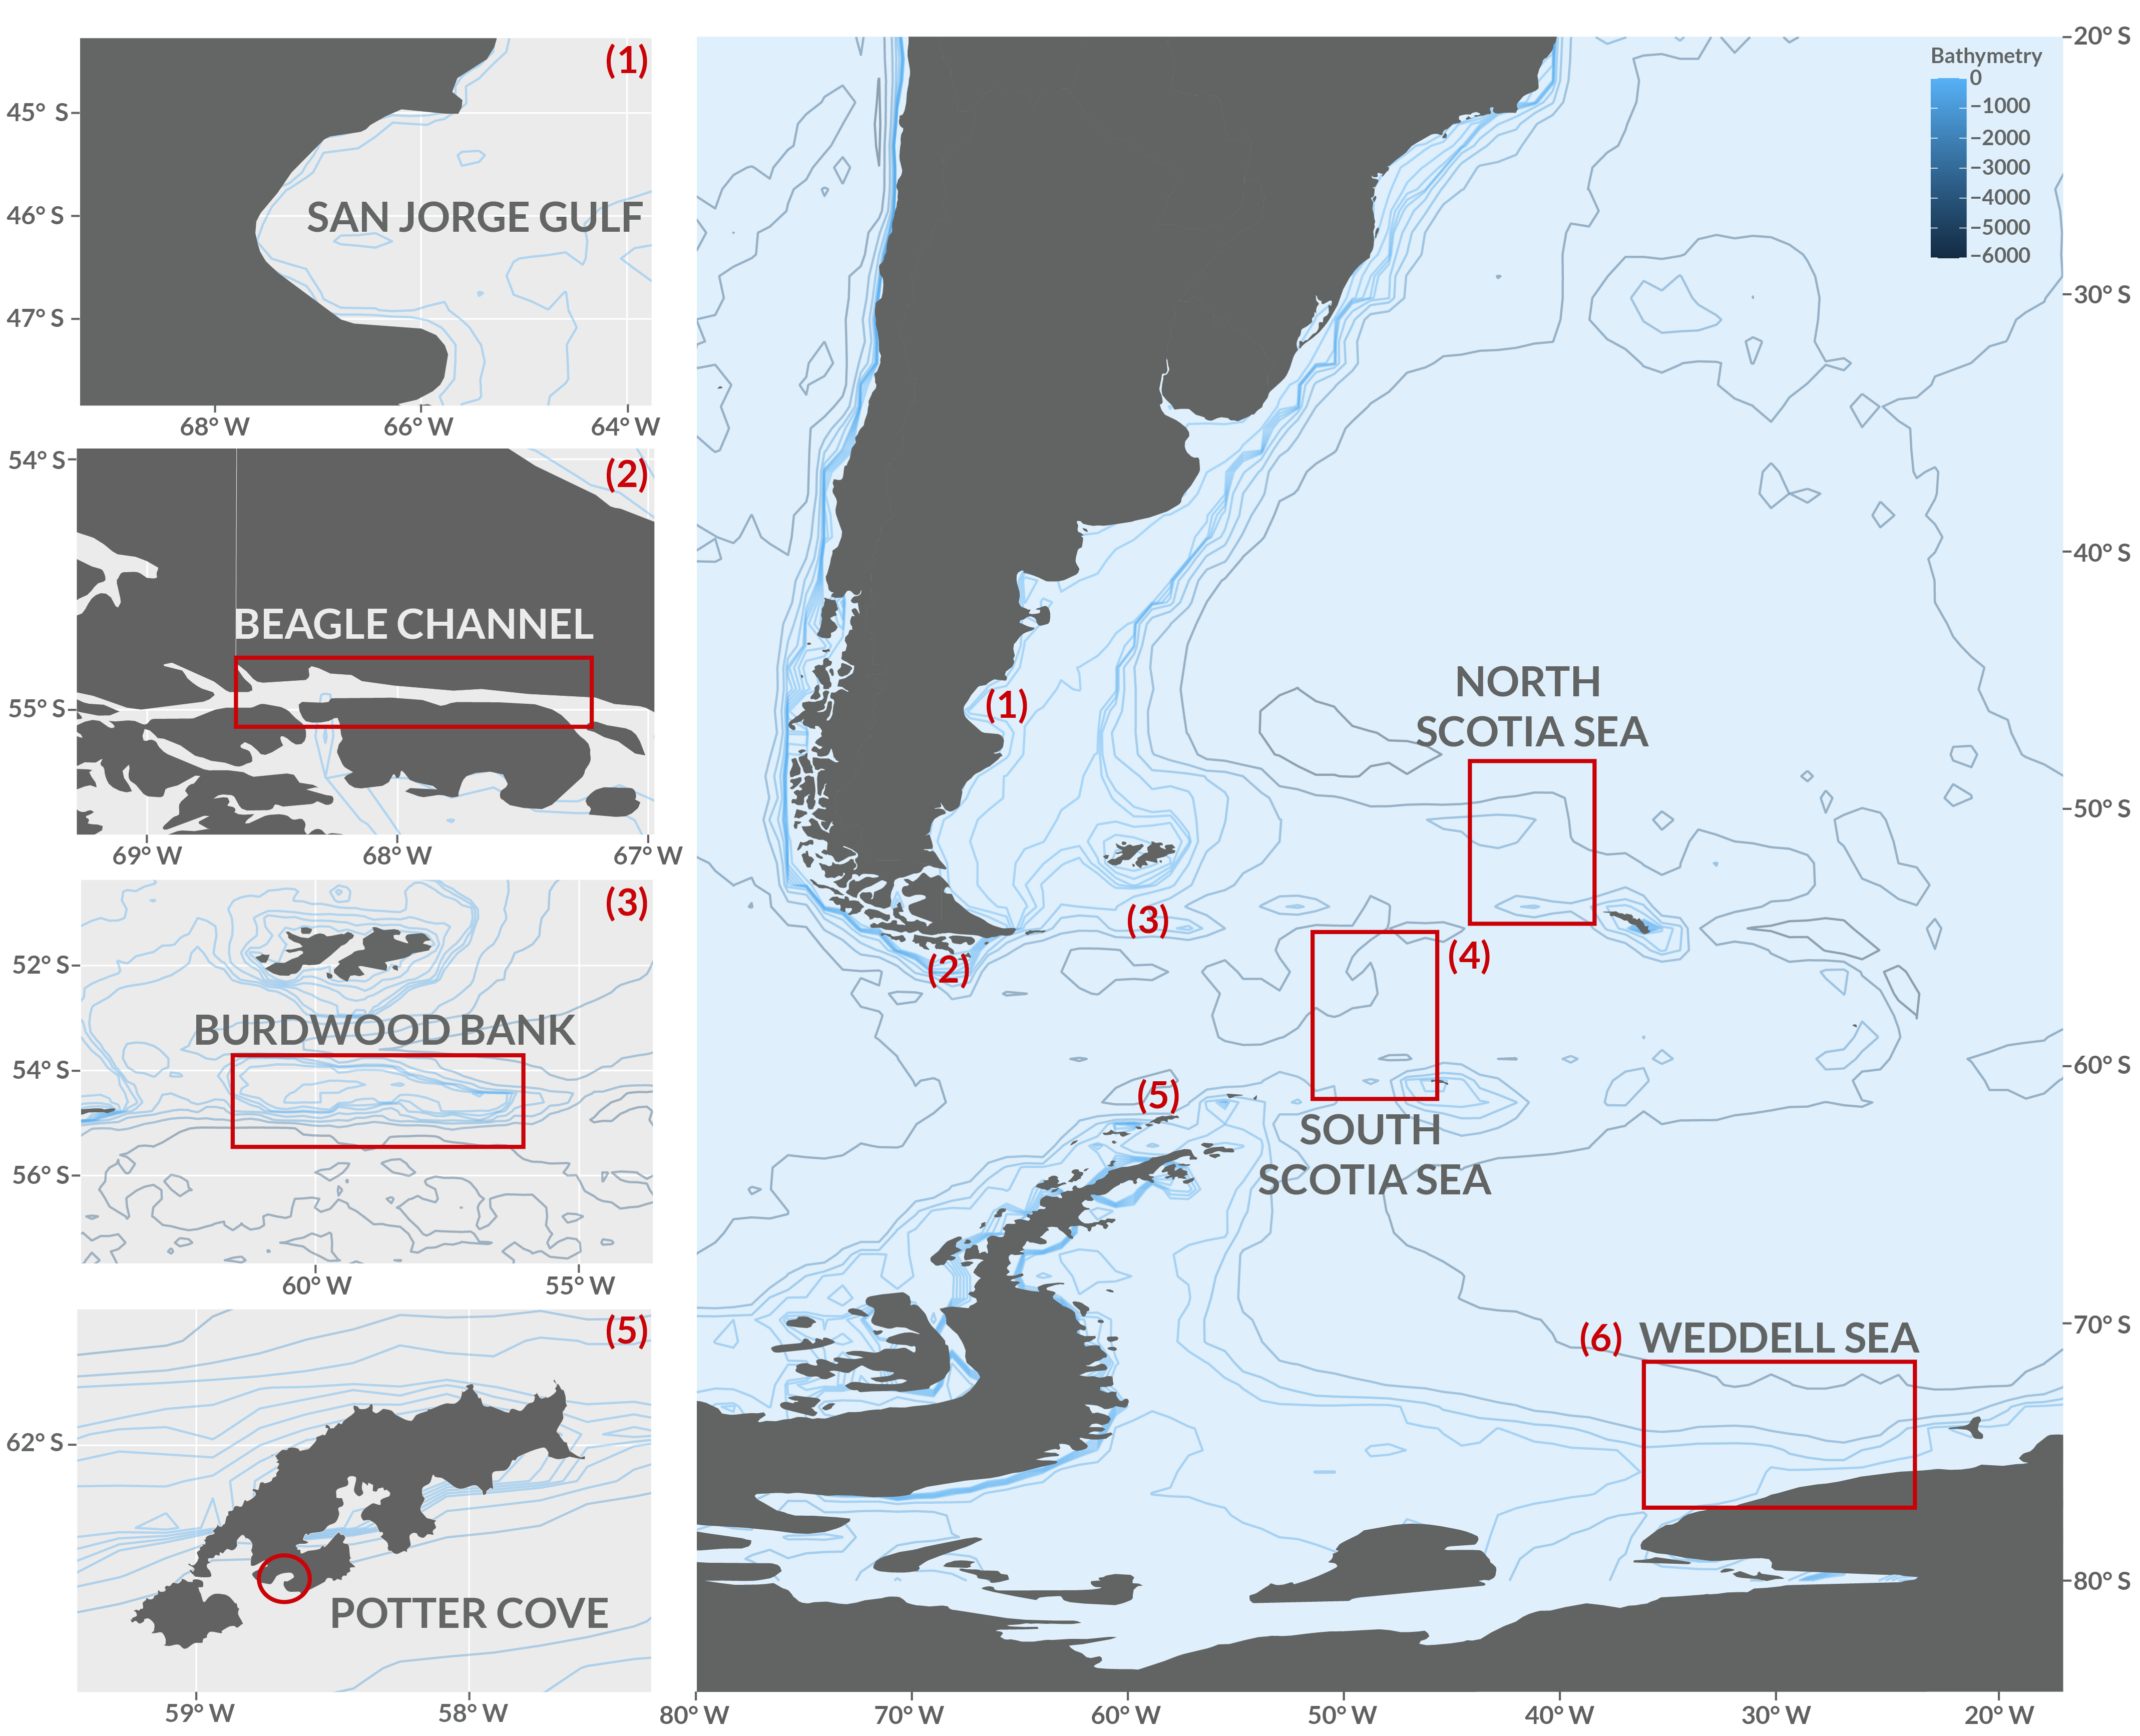
\includegraphics[width=6.27in,height=3.528in]{Figures/Map_final.jpg}
\caption{Map of the study areas along the southwest Atlantic - Antarctic
latitudinal gradient. The areas are marked with numbers from one to six.
Smaller areas (1. San Jorge Gulf, 2. Beagle Channel, 3. Burdwood Bank,
and 5. Potter Cove) are shown on the panels to the left, whereas the
larger areas (4. North and South Scotia Sea, and 6. Weddell Sea) are
marked with a red rectangle on the map. The map was drawn using the
`marmap' R package (Pante et al. 2023). Continental contour shapefiles
were obtained from www.ign.gob.ar.}
\end{figure}

\subsubsection{2.1 San Jorge Gulf}\label{san-jorge-gulf}

San Jorge Gulf is the northernmost study area considered in this review
(Figure 1), located from Cabo dos Bahias (44°55'S) to Cabo tres Puntas
(47°06'S). It is a partially enclosed basin spanning approximately
34,000 \(\text{km}^2\) and \textasciitilde100 m of maximum depths. The
gulf's productivity supports large invertebrate and vertebrate fisheries
(Góngora et al. 2012), as well as marine mammal and seabird populations
(Yorio 2009). Two prominent frontal systems meet in the shallower
northern and southern ends of the gulf (with depths \textasciitilde40
m), which are also the places of highest productivity (Glembocki et al.
2015).

The San Jorge Gulf food web contains 165 nodes (trophospecies) and 1015
trophic interactions with a connectance of 0.04. The percentage of top
predators is 16\%, 78\% of the nodes are intermediate and 6\% are basal;
60\% of the consumers are omnivorous (Table 1). The most connected nodes
are the Argentine red shrimp \emph{Pleoticus muelleri}, the squat
lobster \emph{Gimothea gregaria}, squids (\emph{Illex argentinus} as
dominant species), and Amphipoda. Notably, these nodes are positioned at
mid-trophic levels in the food web (3, 2.5, 3.6, and 2, respectively)
(Funes et al. 2022).

The gulf is subject to several global change stressors (Table 2),
especially fisheries (González-Zevallos and Yorio 2006, 2011; Galván et
al. 2022). By discarding species, trawl fisheries add new trophic
interactions to the food web which results in decreasing trait
variability and stability of the system (Rincón-Díaz et al. 2021; Funes
et al. 2022). Moreover, this has changed the availability of resources
to some predators. For example, the Argentine hake \emph{Merluccius
hubbsi}, one of the main bycatch species, has become a prey item of
non-diving seabirds, like the kelp gull \emph{Larus dominicanus}
(González-Zevallos and Yorio 2006) and reef fish (Funes et al. 2019).
Although juveniles of \emph{M. hubbsi} is largely the main bycatch
species, 29 cartilaginous and 69 bony local fish species were also
registered as incidental catch between 2005 and 2014 (Bovcon et al.
2013; Ruibal Nuñez 2020). This level of impact has triggered a shift in
the functional diversity of fish assemblages in the gulf, homogenizing
their trophic function (Rincón-Díaz et al. 2021), for example in the
sites with the historical highest fishing activity, the fish assemblage
experienced a relative increase in midwater fusiform species and lost
variability in their depth range (Rincón-Díaz et al. 2021). Other
functional changes were a decrease in the maximum sizes of individual
fish, together with a drop in elasmobranch biomass and an increase in
crustacean biomass (Funes 2020). The significant increase in crustacean
biomass was mainly due to the increase in the Argentine red shrimp and
the squat lobster (Funes 2020). These species have become the most
important prey for the most abundant fish in the area, the Argentine
hake and the narrownose smooth-hound \emph{Mustelus schmitti} (Belleggia
et al. 2017; Pasti et al. 2021). However, since commercial fisheries
ceased their activities in the San Jorge Gulf in 2015 (Annex I,
Resolution CFP No 7/2018), the effects mentioned above from trawl
fisheries on the structure and function of the ecosystem may have
changed since then. Nowadays only small-scale trawling from artisanal
fishery is practiced in the gulf. Sea warming is another important
stressor in the San Jorge Gulf, because of the southward shifts of
northern fish populations to the area (Galván et al. 2022). Signs of sea
warming have been detected in the gulf and nearby regions. Anomalous
bottom temperature increments of up to 2°C have been observed in the
gulf since 2000 (Isla and Cortizo 2024), and a positive trend in sea
surface temperature of 0.3°C/0.4°C per decade over a 30-year series
(Saraceno et al. 2022; Risaro et al. 2022). Additionally, a positive
trend in sea surface temperature (\textasciitilde0.5 °C increase in the
last 20 years) has been reported for the Nuevo and San Jose Gulfs, both
located close to and northward of the San Jorge Gulf (Williams and
Nocera 2023). The region is especially prone to be affected by
climate-driven shifts in species ranges because it is situated in the
ecotone of two biogeographic provinces, the Argentine (30°S - 44°S) and
the Magellanic (43°S - 55°S) (Balech and Ehrlich 2008). In addition to
tropicalization from northern fish populations, alien species are also
documented to affect demersal assemblages of fish and macroinvertebrates
in the gulf (Galván et al. 2022). Finally, the gulf is exposed to urban
and industrial pollution (Verga et al. 2020). In particular, there is an
oil monobuoy from which oil manipulation and general oil transport along
the Patagonian coast registered several oil spills and chronic oil
discharges (García-Borboroglu et al. 2008). Other marine systems
impacted by the oil spill have shown extraordinary mortality events for
cetacean (Litz et al. 2014), sea turtles (Wallace et al. 2017), and
important decrease in marine bird populations (Irons et al. 2000) sea
otters (Garrott et al. 1993) and macroalgae (Southward and Southward
1978), with cascading effects throughout the food web (Peterson 2001).

\subsubsection{2.2 Beagle Channel}\label{beagle-channel}

Located at a more southern latitude (\textasciitilde54°S, 68°W), the
Beagle Channel (Figure 1) is an interoceanic passage at the southernmost
tip of South America, spanning 240 km in length and 5 km in width
(\textasciitilde1200 \(\text{km}^2\)), with a depth range of 0 - 140 m.
It features complex coastlines, varying bathymetry, a prevailing
west-to-east circulation pattern, and a significant longitudinal
gradient of glacial freshwater discharge (Schloss et al. 2023). Bruno et
al. (2023) suggests that locally produced suspended particulate organic
matter (mostly composed of phytoplankton) and organic matter accumulated
in the sediments (macroalgae-originated detritus) are the primary food
sources for the marine ecosystem, as opposed to allochthonous materials.

The Beagle Channel food web includes 145 nodes and 1115 trophic
interactions with a connectance of 0.05 (Table 1). This food web is
hypothesized to have a wasp-waist structure (i.e., the structure and
dynamics of the ecosystem are regulated primarily by mid-trophic level
species), where the following species play a crucial role in the
dynamics of the ecosystem: Fueguian sprat \emph{Sprattus fuegensis},
longtail southern cod \emph{Patagonotothen ramsayi}, black southern cod
\emph{P. tessellata}, frogmouth \emph{Cottoperca trigloides}, and squat
lobster \emph{G. gregaria} (Riccialdelli et al. 2020). Moreover, the
squat lobster has been identified as a species linking food web modules
and connecting the entire food web (Rodriguez et al. 2022).

One of the main local stressors in the Beagle Channel is the
introduction of invasive species (Table 2). Salmonidae were introduced
to Tierra del Fuego in the 1930s. Especially, the Chinook salmon
\emph{Oncorhynchus tshawytscha} causes concern. The detection of this
species in Tierra del Fuego dates back to April 2006, and its population
has been expanding since then (Nardi et al. 2019). Being a top predator,
the Chinook salmon can compete for resources with several native
predators in the Beagle Channel (Correa and Gross 2008), but also prey
on them. This is the case for Notothenioids (\emph{Eleginops
maclovinus}, \emph{Patagonotothen tessellata}, \emph{P. cornucola},
\emph{P. sima}, \emph{Paranotothenia magellanica}, \emph{Harpagifer
bispinis}), the Atherinidae \emph{Odontesthes smitti} and \emph{O.
nigricans}, the Fuegian sprat, and larvae of king crabs (\emph{Lithodes
antarcticus} and \emph{Paralomis granulosa}) (Fernández et al. 2010).
Ciancio et al. (2008) observed that Chinook salmon primarily feeds on
sprats in the Southern Patagonian Shelf Ecosystem area and display
trophic levels comparable to those of intermediate-sized fish and
cephalopod predator species, showing significant dietary overlap with
the Magellanic penguin \emph{Spheniscus magellanicus}. Another potential
competitor for Chinook salmon in the Beagle Channel, sharing a similar
diet, is the native Commerson's dolphin \emph{Cephalorhynchus
commersonii} (Riccialdelli et al. 2013). In invaded ecosystems,
predation emerges as the primary driver of significant damage, often
leading to cascading effects impacting even primary producers (David et
al. 2017). In the Beagle Channel, other stressors include contaminants
like metals, perfluorinated compounds, hydrocarbons, and microplastics
found in animal tissue (algae, mussel, fish, and guano) and sediments
(Duarte et al. 2011; Llorca et al. 2012). Carbon and carbohydrate levels
in Ushuaia Bay's (54°48′S, 68°18′W) surface sediments are similar to
hypertrophic ecosystems (i.e., greater input of nutrients than an
eutrophic situation), along with hydrocarbons and heavy metals linked to
port and industrial activities (Gil et al. 2011; Commendatore et al.
2012). Ferreira et al. (2021) showed that the black southern cod in
Ushuaia Bay may be exposed to endocrine-disrupting compounds from urban
and industrial pollution. Moreover, Pérez et al. (2020) and Ojeda et al.
(2021) found microplastics in the Chilean mussel \emph{Mytilus
chilensis} and the sea snail \emph{Nacella magellanica}, respectively.
These studies link pollutants to port and industrial activities of
Ushuaia; we therefore expect the area of the Beagle Channel closest to
the city to be the most affected by contaminants. Contaminants
potentially spread through the food web, from lower to higher trophic
level taxa. In the Beagle Channel and Atlantic coast of Tierra del Fuego
food webs mercury concentrations rose with benthivory, and higher
mercury was found in phytoplankton and the squat lobster. This latter
species connects pelagic and benthic habitats, so any disruption to them
could disrupt the food web (Rodriguez et al. 2022). Dodino et al. (2022)
found the highest mercury levels in Magellanic penguin feathers from
offshore colonies in Tierra del Fuego. Recently, Ushuaia's kelp forests
have also seen changes in composition along with a decrease in
biodiversity as a result of urban pollution (Kaminsky et al. 2023). It
is important to note that sea warming might be a less significant
stressor in the Beagle Channel compared to the other areas, as global
warming is melting glaciers and the influx of cold freshwater is
actually slightly cooling the seawater (Saraceno et al. 2022).

\subsubsection{2.3 Burdwood Bank}\label{burdwood-bank}

The so-called Burdwood Bank ecosystem comprises Marine Protected Areas
Namuncurá - Burdwood Bank I and II (\textasciitilde54°S, 59°W), meaning
the shallow submarine plateau named Burdwood Bank with a 200 m isobath
boundary, and a deep slope that reaches 4000 m in depth, respectively
(Administración de Parques Nacionales 2022) (Figure 1). Physical
features in the plateau are fairly stable, with salinity averaging 34
all year round and temperature ranging between 4 and 8°C (Acha et al.
2004). The plateau is surrounded by steep flanks of up to 4000 m depth,
protected by the Marine Protected Area Namuncurá - Burdwood Bank II
(32,000 \(\text{km}^2\)). Intense upwelling and mixing occur in relation
to the slope, entraining deep nutrient-rich waters into the photic layer
(Matano et al. 2019), and resulting in a fairly homogeneous water column
both spatially and temporally (Matano et al. 2019).

The Burdwood Bank food web comprises 379 nodes and 1788 interactions,
with a connectance of 0.01, and an asymmetric degree distribution
(i.e.~most of the species have a relatively low number of interactions
and few species concentrate most of them). Almost half of the consumers
are omnivores (48\%), and the network displays a small-world pattern
(Marina et al. 2024b) (Table 1). This network pattern implies a rapid
spread of a perturbation (e.g., contaminant, population fluctuation,
local extinction) throughout the food web due to a short distance among
species but, at the same time, a greater resistance caused by the
confinement of perturbations mainly within subnetworks as a result of a
high clustering coefficient (Bornatowski et al. 2017; Dormann et al.
2017).

The main stressors reported for the ecosystem of the Marine Protected
Areas Namuncurá within Burdwood Bank I and II are related to human
activities such as fisheries and contamination (Table 2). Several
fisheries targeting demersal fish operate in the vicinity and within the
Marine Protected Areas. The fishery of the Patagonian toothfish
\emph{Dissostichus eleginoides} has gained prominence in recent years
(Allega et al. 2020; Gorini et al. 2021). Although these are regulated
by the Argentinean government, incidental bycatches do occur, where
demersal fish of the genera \emph{Coelorinchus} and \emph{Macrourus},
seabirds and benthic invertebrates (30+ taxa) are the most common
bycatches (Gaitán and Marí 2016; Martínez et al. 2022). Noteworthy,
among the invertebrates caught, eight species are indicator taxa of
vulnerable marine ecosystems (Gaitán and Marí 2016; Schejter and Albano
2021). However, independent assessments of these bycatches suggest no
significant impact on the populations (Gaitán and Marí 2016; Martínez et
al. 2022). Besides bycatches, seabirds are being affected by fisheries
due to discards, altering their diet; the most frequently encountered
species are black-browed albatross \emph{Thalassarche melanophris},
Southern giant petrel \emph{Macronectes giganteus}, Cape petrel
\emph{Daption capense}, Southern royal albatross \emph{Diomedea
epomophora}, Northern giant petrel \emph{M. halli}, and white-chinned
petrel \emph{Procellaria aequinoctialis} (Tamini et al. 2023).
Nevertheless, there is a lack of knowledge considering their role in the
ecosystem and the potential joint effect of both target fish and bycatch
in a broader food web framework. Contaminants such as microplastics and
mercury occur in the water column of the Burdwood Bank ecosystem (Cossi
et al. 2021; Fioramonti et al. 2022; Di Mauro et al. 2022).
Microplastics are distributed along the entire water column, from
surface to deep waters (3-2450 m) (Di Mauro et al. 2022). More
importantly, microplastics were found in soft tissues of benthic
macroinvertebrates (sea stars \emph{Henricia obesa} and \emph{Odontaster
penicillatus}) and benthopelagic fish (\emph{Patagonotothen guntheri}
and \emph{P. ramsayi}), which not only incorporated the contaminant from
the environment through their filter-feeding system but could also get
it indirectly from prey organisms already containing plastics in their
tissues (Cossi et al. 2021). Notably, one of the contaminated species is
the longtail southern cod \emph{P. ramsayi}. This species is part of the
core group of species that drive the ecosystem through the suggested
wasp-waist control (Riccialdelli et al. 2020). Mercury transfer and
biomagnification are occurring at a greater pace than near coastal areas
such as the Beagle Channel (Fioramonti et al. 2022). The Fuegian sprat
\emph{S. fuegensis}, a pelagic fish with a mid-trophic level in the food
web, has the highest levels of mercury recorded (Fioramonti et al.
2022). Considering the wasp-waist control of the Fuegian sprat in the
food web (Riccialdelli et al. 2020), a rapid and widespread
contamination to the top predators is expected (Fioramonti et al. 2022).
Despite evidence of warming of surface, mid-water and bottom layers (100
m) in Burdwood Bank (Franco et al. 2020a), studies on the oceanographic
aspects of the system are lacking. Warming impacts on the species and
trophic interactions in Burdwood Bank are also unknown.

\subsubsection{2.4 Scotia Sea}\label{scotia-sea}

The Scotia Sea is a deep-sea basin (\textasciitilde48 - 58°S, 50°W),
delimited by the Drake Passage to the West and by the island complex of
the Scotia Arc to the North, East, and South, with an approximate
extension of 1.5 x 106 \(\text{km}^2\) and a depth range of 0 - 3000 m
(Murphy et al. 2006) (Figure 1). Its oceanography is dominated by the
Antarctic Circumpolar Current, which is spatially structured by frontal
systems (Whitworth 1980). The South Antarctic Circumpolar Current Front
subdivides the Scotia Sea into two biogeographic regions: the Northern
Scotia Sea, characterized by higher and more variable temperatures, and
the Southern Scotia Sea, characterized by lower and more stable
temperatures and influenced by seasonal sea ice (Raymond 2011).

Analysis of the Northern and Southern Scotia Sea food webs shows that
the former is relatively more complex in terms of number of species and
links than the latter: with more species richness (218 vs 192) and
interactions (10008 vs 7241) and a slightly higher connectance (0.21 vs
0.20). Mean path length is shorter in the Northern Scotia Sea food web,
whereas the Southern Scotia Sea network displays a greater proportion of
omnivores and a lower mean trophic level (López-López et al. 2022)
(Table 1).

The Scotia Sea is a vast and heterogenous oceanic region, where
especially the zone around South Georgia island represent an area of
interest, here referred to as `Northern Scotia Sea'. The majority of
studies analyzing the stressors' effects come from this area (e.g.,
Murphy et al. (2007); Whitehouse et al. (2008); Trathan (2023)) (Table
2). The main stressor of the Scotia Sea is commercial fisheries. Krill
fishery on \emph{Euphausia superba} not only impacts the targeted
species, but also the many predators that depend on it as a food source
(Hilborn et al. 2017). Yet, data currently available from monitoring of
krill and its predators remain insufficient, hence identifying the
potential fishery impacts on the ecosystem is difficult (Trathan et al.
2021). Apart from krill fishery, two other commercial fisheries operate
in the Scotia Sea, targeting Patagonian toothfish species \emph{D.
eleginoides} and \emph{Dissostichus mawsoni}. The \emph{D. eleginoides}
stock is linked to the stock at South Georgia (`Northern Scotia Sea')
(Collins et al. 2010), while the \emph{D. mawsoni} stock is linked to
the Antarctic continental shelf (`Southern Scotia Sea') (Soeffker et al.
2022). Recently, Trathan (2023) has identified several concerns
regarding aspects of these fisheries, highlighting that it is crucial to
recognize ongoing changes such as the recovery of baleen whales and
climate change. These factors increase the uncertainty for fishery
managers, necessitating direct consideration in the management of
harvested and dependent species.

The Scotia Sea has experienced one of the largest levels of warming
within the polar regions (Whitehouse et al. 2008). Together with the
Southern Annular Mode anomalies, this has caused a long-term decrease in
krill abundance; more pronounced in the northern than in the southern
Scotia Sea (Murphy et al. 2007). Over the past 90 years, the Antarctic
krill \emph{E. superba} also showed an increase in mean body length
(Atkinson et al. 2019), likely altering predator-prey interactions.
Moreover, it allows krill to reach colder feeding grounds near the
seabed, with the potential to link krill to unexpected predators such as
demersal fish (Schmidt et al. 2011). Because of warming, the krill
distribution has shifted southward (Atkinson et al. 2019), changing the
food web from a krill-based to a non-krill-based, where myctophid fish
and squid are playing important roles as key species in a wasp-waist
controlled system (Saunders et al. 2019). While the krill distribution
has shifted southward, the most abundant calanoid copepods have
maintained their distribution (Tarling et al. 2018). Mercury transfer
and biomagnification are current processes occurring in the Scotia Sea,
where the total concentration of contaminants increase with trophic
level and are highest in notothenioid and myctophid fish (e.g.~\emph{D.
eleginoides}, \emph{Gymnoscopelus nicholsi}), and seabirds (Seco et al.
2021). During years of low Antarctic krill abundance, predators must
deal with both the stress of reduced prey availability and the
concurrent rise in mercury exposure (Seco et al. 2021).

\subsubsection{2.5 Potter Cove
(Antarctica)}\label{potter-cove-antarctica}

In the Antarctic realm, Potter Cove is a \textasciitilde9
\(\text{km}^2\) fjord with a depth range of 0 - 200 m located at 25 de
Mayo/King George Island (62°S, 58°W) on the South Shetland Islands of
the West Antarctic Peninsula (Figure 1). The cove, bordered by the
Fourcade Glacier, is divided into three areas: a) the internal cove, a
high glacier-influenced, soft sediment zone with a 50 m maximum depth;
b) the central cove, a mixed substrate area with low meltwater influence
and an 80 m maximum depth; and c) the external cove, ice-free for 60
years with a 185 m maximum depth and rocky substrate (Jerosch et al.
2018). Potter Cove's high-latitude location results in variable
environmental conditions due to photoperiod length seasonality. Sea ice
often covers this area in winter (Schloss et al. 2012). With low
phytoplankton biomass, macroalgae, and microphytobenthos are likely the
primary food sources for secondary benthic production (Quartino and
Boraso de Zaixso 2008).

The Potter Cove food web includes 110 nodes and 649 interactions, and a
connectance of 0.05 (Table 1). It presents an asymmetric degree
distribution and a modular structure, i.e., groups of species interact
more strongly with each other within modules than with species belonging
to other modules (Rodriguez et al. 2022).

Regional warming in the West Antarctic Peninsula recorded in the last
half-century (Chown et al. 2022) has been one of the main stressors
driving changes in Potter Cove (Table 2), a system highly dependent on
glacier and sea ice dynamics (Deregibus et al. 2017). This has caused
drastic environmental and biological transformations such as shifts in
dominance within the benthic community (Schloss et al. 2012; Quartino et
al. 2013; Sahade et al. 2015). In Potter Cove, there has been a
decreasing trend in total sea ice cover since 1991 (Schloss et al.
2012). Changes in the annual timing of landfast ice formation and the
breakup of the sea ice cover has multiple effects on species (Michel et
al. 2019). Warmer winters and springs result in earlier sea ice melt,
causing an abrupt increase in the light available for benthic primary
producers (Deregibus et al. 2020). Sea ice also mediates physical
disturbances to the benthos by influencing sedimentation and iceberg
scouring. These factors affect the production of macroalgae, albeit in
opposite ways (Deregibus et al. 2017), and microphytobenthos (Hoffmann
et al. 2019). On the other hand, sea ice is an important habitat for
diatoms and their associated consumers, including copepods and the
Antarctic krill (Flores et al. 2012), and thus important for
bentho-pelagic nutrient and carbon cycling during winter. Additionally,
a decrease in winter sea ice cover produces an increase in physical
perturbation on benthic shallow communities in coastal shallows due to
ice scouring (Deregibus et al. 2017). The glacier surrounding Potter
Cove has been receding at an increasing rate since 1950 (Rückamp et al.
2011), which has caused a massive discharge of sediment-laden meltwater
(Meredith et al. 2018). Large quantities of suspended particles affect
growth, survival, and reproduction of benthic species. This led to a
major shift in the benthic community structure, from a filter
feeders--ascidian domination to a mixed assemblage with scavengers and
opportunistic species (Sahade et al. 2015), and the metabolic balance in
benthos went from net autotrophy to heterotrophy (Braeckman et al.
2021). Additionally, massive stranding events of the tunicate
\emph{Salpa thompsoni} and the Antarctic krill linked to the presence of
glacial meltwater have been reported (Fuentes et al. 2016). Rising
temperatures leading to ice and glacial melting has also substantial
impacts on pelagic primary productivity, since it reduces water
salinity, affecting water column stratification, light penetration and
nutrient availability for photosynthesis (Schloss et al. 2012). In
Potter Cove, changes in biomass of most phytoplankton species have been
observed under heat wave conditions, resulting in a shift from a
microplankton to a nanoplankton dominated community (Antoni et al. 2020;
Latorre et al. 2023). This means that in areas strongly affected by
glacier melt, the planktonic food web is dominated by the microbial loop
(i.e., ciliates and heterotrophic dinoflagellates preys upon
nanophytoplankton, which are sequentially available prey for small
omnivorous copepods), instead of being predominantly herbivorous (Garcia
et al. 2016, 2019). In addition, phytoplankton species under these
warming conditions showed a decrease in metabolic rate and in the
quality of the fatty acid composition (Latorre et al. 2023).

\subsubsection{2.6 Weddell Sea
(Antarctica)}\label{weddell-sea-antarctica}

Located between 74 and 78°S, the high Antarctic Weddell Sea shelf spans
approximately 450 km from East to West (Jacob et al. 2011) (Figure 1).
The water depth ranges from 200 to 500 m, with shallower regions being
covered by continental ice that forms the coastline along the eastern
and southern parts of the Weddell Sea. The shelf area is characterized
by a complex three-dimensional benthic habitat, substantial benthic
biomasses, and an intermediate to high diversity (Teixidó et al. 2002).

The Weddell Sea food web exhibits a high level of network complexity,
featuring the greatest number of nodes (490) and trophic interactions
(16041) among the marine food webs of the Southern Hemisphere (Table 1).
Its connectance (0.07), mean trophic level (2.62) and omnivory (51\%)
are intermediate compared to the other food webs (Table 1). Recently,
the interaction strengths of this food web were estimated, revealing the
presence of numerous weak and few strong interactions (Marina et al.
2024a).

In the Weddell Sea, the main stressors are related to warming impacts
(sea warming, sea ice extent, iceberg scouring) (Table 2), where sea
warming has been substantial since the early 1980s (Turner et al. 2020).
For example, in 2017, the mean temperature for February reached 1.45°C,
the highest monthly mean ever recorded, i.e., 0.56°C above the
climatological mean (Turner et al. 2020). Warming has caused spatial and
temporal reductions in sea ice, impacting both pelagic and benthic
communities (Constable et al. 2014; Gutt et al. 2021). Since the start
of satellite imaging in 1978, sea ice extent has reached new record
lows. Some of the most pronounced impacts of decreasing sea ice are
negative changes in primary productivity (Atkinson et al. 2004) and
declines of the Antarctic krill. Moreover, reduced sea ice cover allows
increased access to krill by its predators (Kawaguchi et al. 2009),
which further contributes to its decline. Some outcomes of the krill
decline are reduced energy intake by higher trophic levels such as
humpback whales \emph{Megaptera novaeangliae} Braithwaite et al. (2015)
which rely heavily on krill for foraging, as well as reduced carbon
export due to fewer fecal pellets (Pauli et al. 2021). Many higher
trophic level species in the Weddell Sea are greatly impacted by sea ice
reductions due to loss of habitat and food source availability, such as
the Antarctic petrel \emph{Thalassoica antarctica} - one of the most
abundant seabirds in the Weddell Sea (Orgeira et al. 2021). Other
impacted sea bird species are the emperor penguin \emph{Aptenodytes
forsteri}. Reductions in sea ice constrain its population as evidenced
by recent observations in the Bellingshausen Sea region (Fretwell et al.
2023). The Arctic tern \emph{Sterna paradisaea} spends the summer in the
Weddell Sea exploiting krill swarms under receding ice edges. Thus,
continued warming is expected to gradually erode the abundance and
distribution of marine seabirds in the Weddell Sea (Orgeira et al.
2021). Many marine mammals depend on for breeding and foraging such as
the Weddell and Crabeater seals (\emph{Leptonychotes weddellii} and
\emph{Lobodon carcinophagus}) (Wege et al. 2021) and the Humpback whale.
Reduced sea ice can significantly affect the breeding success of seals
(Wege et al. 2021) and body condition of whales (Turner et al. 2020).
Notothenioid fish, with \emph{Pleuragramma antarcticum} being the most
abundant species, confront numerous stressors such as sea warming, sea
ice decline, and ocean acidification, posing significant threats to
their survival. While certain species exhibit physiological plasticity
to cope with increased oxygen demand, most notothenioid fish are
stenothermal and incapable of adjusting their metabolic functioning
(Mintenbeck et al. 2012). Projections suggest that the preferred thermal
habitat of the Antarctic toothfish, \emph{Dissostichus mawsoni}, an
important fish species in the Weddell Sea ecosystem, may contract over
the next three decades, underscoring the potential impact of global
warming on these species (Constable et al. 2014). Iceberg scouring is a
major factor in driving the high biodiversity of benthic communities in
the Weddell Sea (Gutt and Starmans 2001). Even at 600 m depths, iceberg
scouring has a strong effect on the benthic environment, disrupting the
upper layers of the seabed and removing macrofauna. This patchy
disturbance and distribution pattern occurs roughly every 200 square
meters on the Antarctic continental shelf. Global warming is predicted
to increase iceberg scouring frequency (Gutt 2001; Smale et al. 2008),
disrupting the environment (Smale and Barnes 2008) with the potential
for tipping points (Gutt et al. 2015).

\newpage
\footnotesize

Table 1. Complexity and structure properties of the marine food webs
considered in the present review. Refer to Table S2 for definition of
properties. mean TL: mean trophic level. Food webs are ordered by
increasing latitude.

\begin{longtable}[]{@{}
  >{\raggedright\arraybackslash}p{(\columnwidth - 14\tabcolsep) * \real{0.1538}}
  >{\centering\arraybackslash}p{(\columnwidth - 14\tabcolsep) * \real{0.0839}}
  >{\centering\arraybackslash}p{(\columnwidth - 14\tabcolsep) * \real{0.0839}}
  >{\centering\arraybackslash}p{(\columnwidth - 14\tabcolsep) * \real{0.1259}}
  >{\centering\arraybackslash}p{(\columnwidth - 14\tabcolsep) * \real{0.1259}}
  >{\centering\arraybackslash}p{(\columnwidth - 14\tabcolsep) * \real{0.0979}}
  >{\centering\arraybackslash}p{(\columnwidth - 14\tabcolsep) * \real{0.1049}}
  >{\centering\arraybackslash}p{(\columnwidth - 14\tabcolsep) * \real{0.2238}}@{}}
\toprule\noalign{}
\begin{minipage}[b]{\linewidth}\raggedright
\textbf{Food web}
\end{minipage} & \begin{minipage}[b]{\linewidth}\centering
\textbf{Nodes}
\end{minipage} & \begin{minipage}[b]{\linewidth}\centering
\textbf{Links}
\end{minipage} & \begin{minipage}[b]{\linewidth}\centering
\textbf{Connectance}
\end{minipage} & \begin{minipage}[b]{\linewidth}\centering
\textbf{Path length}
\end{minipage} & \begin{minipage}[b]{\linewidth}\centering
\textbf{mean TL}
\end{minipage} & \begin{minipage}[b]{\linewidth}\centering
\textbf{Omnivory}
\end{minipage} & \begin{minipage}[b]{\linewidth}\centering
\textbf{Reference}
\end{minipage} \\
\midrule\noalign{}
\endhead
\bottomrule\noalign{}
\endlastfoot
San Jorge Gulf & 165 & 1015 & 0.04 & 2.17 & 3.02 & 0.63 & Funes et al.
(2022) \\
Beagle Channel & 145 & 1115 & 0.05 & 2.12 & 2.37 & 0.55 & Rodriguez et
al. (2022) \\
Burdwood Bank & 379 & 1788 & 0.01 & 2.99 & 2.52 & 0.49 & Marina et al.
(2024b) \\
Potter Cove & 110 & 649 & 0.05 & 2.33 & 2.22 & 0.46 & Marina et al.
(2018); Rodriguez et al. (2022) \\
N Scotia Sea & 218 & 10008 & 0.21 & 1.87 & 3.29 & 0.73 & López-López et
al. (2022) \\
S Scotia Sea & 192 & 7241 & 0.20 & 1.90 & 3.21 & 0.71 & López-López et
al. (2022) \\
Weddell Sea & 490 & 16041 & 0.07 & 2.19 & 2.62 & 0.51 & Jacob et al.
(2011) \\
\end{longtable}

\normalsize

\subsection{3. From species' stressors to food web effects: a
qualitative
approach}\label{from-species-stressors-to-food-web-effects-a-qualitative-approach}

A major challenge in contemporary ecology lies in predicting the effects
of stressors on complex multispecies systems, such as food webs. Network
analysis has proved to be a powerful tool to tackle this issue, since it
can capture the effects of individual and multiple stressors on
communities and ecosystems (Montoya et al. 2009; O'Gorman et al. 2012;
Bruder et al. 2019).

Global change stressor effects in the Southwest and the Atlantic sector
of the Southern Ocean have been mostly assessed individually and at the
organism and/or population, i.e., at the node level (Table 2), with one
exception: the effect of fisheries in the San Jorge Gulf food web (see
section below for more details). To address the most plausible effects
of the main stressors on the selected food webs, given the current
information, we formulated a series of alternative hypotheses for each
study area. To this aim, we developed a theoretical framework
considering the following: a) stressor(s), b) parameter(s) affected, c)
node-level properties of the affected species, and d) network-level
properties of the food web.

We considered that a stressor will affect one of the following species'
characteristics or parameters: metabolism, population biomass,
distribution, and diet (Figure 2). `Metabolism' refers to any change
related to metabolic rate, such as reproduction, hatching, larval
development, growth and mortality (e.g.~growth effect in filter-feeders
due to sediment in water column in Potter Cove; endocrine disruption in
fish due to urban pollutants in Beagle Channel). `Population biomass'
indicates an effect at the population level, where the density/abundance
is being impacted (e.g.~abundance decreases in macrobenthos due to
iceberg scouring in Weddell Sea). `Distribution' entails a change at the
population level in the geographic space occupied by a species,
e.g.~southward contraction of Antarctic krill due to sea warming of the
Scotia Sea. `Diet' includes alterations in the prey items of a species
at the population level, e.g, due to prey switching, having a direct
effect on the structure of the food web, e.g.~new prey item (discards)
for seabirds due to fishery activities in Burdwood Bank. Next, we
considered node- and network-level properties relevant to the
hypothesized stressor effects on the food webs, and which have been
previously calculated for the studied food webs (Table 2). At the
node-level, we included: a) degree, b) trophic position, c) omnivory
index, and d) relative abundance (see Table S1 in Supporting Information
for properties of stressed nodes). At the network-level, we considered:
a) connectance, b) path length, c) mean trophic level, and d) omnivory
(Table 1).

\begin{figure}
\centering
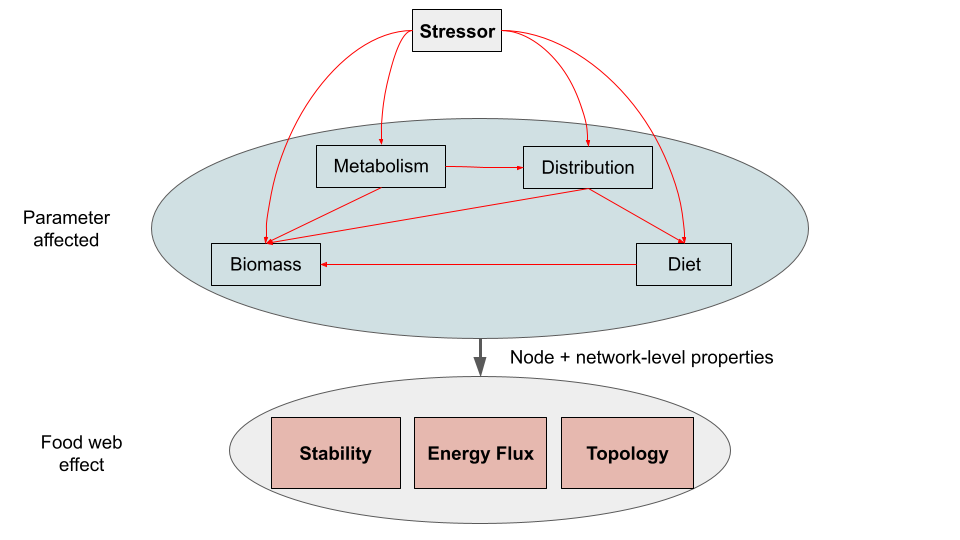
\includegraphics[width=6.27in,height=3.528in]{Figures/Figure2_StressorDiagram.png}
\caption{Conceptual diagram: from species' stressors to food web
effects. A stressor (e.g., global warming) will affect one of the
following species' characteristics: metabolism, population biomass,
distribution, and diet. `Metabolism' refers to any change related to
metabolic rate, such as reproduction, hatching, larval development,
growth and mortality, and contamination due to pollutants. `Population
biomass' indicates an effect at the population level, where the
density/abundance is being impacted. `Distribution' entails a change at
the population level in the geographic space occupied by a species.
`Diet' includes alterations in the prey items of a species at the
population level. Next, we considered node- and network-level properties
relevant to the hypothesized stressor effects on the food webs. At the
node-level, we included: a) degree, b) trophic position, c) omnivory
index, and d) relative abundance. At the network-level, we considered:
a) connectance, b) path length, c) mean trophic level, and d) omnivory.
Finally, we elaborate a series of competing hypotheses on how the
identified stressors might affect food web features (stability, energy
flow, topology), combining information on node- and network-level
properties.}
\end{figure}

\newpage
\begin{landscape}
\scriptsize

Table 2. Environmental and anthropogenic stressors reported for the
study areas: San Jorge Gulf, Beagle Channel, Burdwood Bank, Scotia Sea
(North and South), Potter Cove, and Weddell Sea. Stressor categories:
sea warming; glacial retreat; sediment in the water column; iceberg
scouring; sea ice extent; ocean acidification; ocean acidification +
plastics; microplastics; mercury; urban \& industrial pollution;
fishery; alien species. The species affected were considered at the node
level, whereas effects were considered at the organism and population
levels. Categories of affected parameters and variables: metabolism;
biomass; distribution; diet (see text for explanation). ``Locality''
indicates whether a stressor for a given species was reported for the
study area (`In situ') or in another area (`Elsewhere').

\newcolumntype{L}[1]{>{\raggedright\arraybackslash}p{#1}}
\newcolumntype{C}[1]{>{\centering\arraybackslash}p{#1}}
\newcolumntype{R}[1]{>{\raggedleft\arraybackslash}p{#1}}

\begin{longtable}{ L{2.1cm} L{2.5cm} L{4cm} L{2.5cm} L{2cm} L{3cm} }
\hline
\textbf{Study area} & \textbf{Stressor} & \textbf{Species affected} & \textbf{Parameter affected} & \textbf{Locality} & \textbf{Reference} \\
\hline
\endhead
\endfoot
\hline
\endlastfoot
\textbf{San Jorge Gulf} & & & & & \\
& Sea warming & Fish assemblage \& its prey & Distribution & In situ &
Galván et al. (2022) \\
& Fishery & Demersal fish community & Biomass & In situ & Galván et al.
(2022) \\
& Fishery & Macroinvertebrates, fish and seabirds Di & et In & situ
(\textbf{G?}) & onzalez-Zevallos2006; González-Zevallos and Yorio
(2011); Yorio et al. (2017) \\
& Alien species & Fish assemblage \& its prey & Distribution & In situ &
Galván et al. (2022); Ciancio et al. (2010) \\
& Urban \& industrial pollution & Seabirds \& benthic assemblage &
Biomass & Elsewhere & Moore and Dwyer (1974); Buskey et al. (2016) \\
\textbf{Beagle Channel} & & & & & \\
& Urban \& industrial pollution & Macroalgae; Mytilus edulis chilensis,
Patagonotothen tessellata & Metabolism & In situ & Giarratano and Amin
(2010); Ferreira et al. (2021); Kaminsky et al. (2023) \\
& Mercury & Phytoplankton, Zooplankton, \emph{Grimothea gregaria} &
Metabolism & In situ & Fioramonti et al. (2022) \\
& Microplastics & Mytilus edulis chilensis, Nacella magellanica &
Metabolism & In situ & Pérez et al. (2020); Ojeda et al. (2021) \\
& Alien species: Chinook salmon Oncorhynchus tshawytscha &
Patagonotothen tessellata, Sprattus fuegensis & Diet/Biomass & In situ
(the presence), Elsewhere (changes in prey biomass) & Fernández et al.
(2010); Ciancio et al. (2008) \\
\textbf{Burdwood Bank} & & & & & \\
& Mercury & Dissostichus eleginoides, Sprattus fuegensis, Patagonotothen
ramsayi, Cottoperca trigloides (fish) \& squids Me & tabolism In & situ
(\textbf{F?}) & ioramonti2022 \\
& Microplastics & Henricia obesa \& Odontaster penicillatus (sea stars);
Patagonotothen guntheri \& P. ramsayi (fish) Me & tabolism In & situ
(\textbf{C?}) & ossi2021; Pérez et al. (2021) \\
& Fishery & Target: Dissostichus eleginoides. Bycatch: Macrourus sp.,
Coelorinchus sp. (fish), Daption capense, Thalassarche melanophris,
Macronectes giganteus, T. chrysostoma, Diomedea epomophora (seabirds),
30+ spp macrobenthos Bi & omass El & sewhere (\textbf{G?}) & aitan2016;
Martínez et al. (2022); Administración de Parques Nacionales (2022);
Tamini et al. (2023) \\
& Fishery & Thalassarche melanophris, Macronectes giganteus, Daption
capense, Diomedea epomophora, M. halli, Procellaria aequinoctialis
(seabirds) & Diet & Elsewhere & Tamini et al. (2023) \\
\textbf{Scotia Sea, North \& South} & & & & & \\
& Mercury & Krefftichthys anderssoni, Protomyctophum bolini, Electrona
antarctica, Gymnoscopelus nicholsi, Gymnoscopelus braueri, Dissostichus
eleginoides & Metabolism & In situ & Seco et al. (2021) \\
& Ocean acidification + plastics & Euphausia superba, Limacina
retroversa (Pteropoda) & Metabolism & In situ & Rowlands et al. (2021);
Manno et al. (2022) \\
& Sea warming & Euphausia superba & Metabolism & In situ & Murphy et al.
(2007); Perry et al. (2020) \\
& Sea warming & Euphausia superba & Distribution & In situ & Atkinson et
al. (2019) \\
& Fishery & Euphausia superba & Biomass & In situ & Trathan et al.
(2021) \\
\textbf{Potter Cove (Antarctica)} & & & & & \\
& Sediment in water column & Microphytobenthos, macroalgae, benthic
filter feeders (ascidians), pelagic filter feeders (krill, salps) &
Metabolism & In situ & Sahade et al. (2015); Deregibus et al. (2016);
Fuentes et al. (2016); Hoffmann et al. (2019) \\
& Sea ice extent & Krill & Biomass & Elsewhere & Flores et al. (2012) \\
& Sea ice extent & Benthic community (macroalgae, invertebrates) &
Metabolism & Elsewhere & Clark et al. (2013); Campana et al. (2018) \\
& Glacial retreat & Benthic community (macroalgae, invertebrates) &
Biomass & In situ & Quartino et al. (2013); Lagger et al. (2017); Lagger
et al. (2018) \\
& Iceberg scouring & Benthic community & Biomass & In situ & Deregibus
et al. (2017); Deregibus et al. (2023) \\
& Sea warming & Phytoplankton & Metabolism, biomass & In situ & Antoni
et al. (2020); Latorre et al. (2023) \\
& Sea warming & Zooplankton & Metabolism, biomass, diet & In situ &
Garcia et al. (2016); Garcia et al. (2019) \\
& Sea warming & Fish & Metabolism & In situ, elsewhere & Strobel et al.
(2013); Souza et al. (2018); Saravia et al. (2021) \\
\textbf{Weddell Sea (Antarctica)} & & & & & \\
& Iceberg scouring & Macrobentos & Biomass & In situ & Isla (2023); Gutt
et al. (2015); Smale et al. (2008); Gutt et al. (1996) \\
& Iceberg scouring & Hexactinellida sponges & Biomass & In situ & Gutt
and Starmans (2001); Pineda-Metz et al. (2020); Gutt (2001); Gutt and
Piepenburg (2003) \\
& Ocean acidification & Primary producers / krill / foraminifera /
flagellates & Metabolism & Elsewhere & Deppeler et al. (2020); Isla
(2023); Gutt et al. (2015); Moy et al. (2009) \\
& Ocean acidification & Euphausia superba, Pleuragramma antarcticum &
Metabolism & In situ & Kawaguchi et al. (2010); Kawaguchi et al. (2013);
Piñones and Fedorov (2016); Mintenbeck et al. (2012) \\
& Sea warming & Large (diatoms) \& small (cryptophytes) phytoplankton,
zooplankton (salps) & Metabolism & Elsewhere & Isla (2023); Gutt et al.
(2015); Trebilco et al. (2020) \\
& Sea warming & Euphausia superba, Nototheniid fish, Pleuragramma
antarcticum Me & tabolism In & situ (\textbf{M?}) & eyer2017; Hill et
al. (2013); Mintenbeck et al. (2012); Constable et al. (2014);
Mintenbeck et al. (2012) \\
& Sea ice extent & Phytoplankton, Lobodon carcinophaga, Hydrurga
leptonyx, Leptonychotes weddellii, Ommataphoca rossii, Mirounga leonina,
Arctocephalus gazella & Metabolism & In situ & Pineda-Metz et al.
(2020); Wege et al. (2021); Siniff et al. (2008) \\
& Sea ice extent & Euphausia superba, Pleuragramma antarcticum,
Pagodroma nivea, Thalassoica antarctica, Pygoscelis adeliae & Metabolism
& In situ & Orgeira et al. (2021); Braithwaite et al. (2015); Hill et
al. (2013); Mintenbeck et al. (2012) \\
& Sea ice extent & Megaptera novaeangliae & Metabolism & Elsewhere &
Pallin et al. (2023) \\
& Sea ice extent & Aptenodytes forsteri & Metabolism & Elsewhere &
Orgeira et al. (2021) \\
\end{longtable}

\end{landscape}

\normalsize

\subsubsection{3.1 Hypotheses on the main stressor effects in food webs
in a southwest Atlantic - Antarctic
gradient}\label{hypotheses-on-the-main-stressor-effects-in-food-webs-in-a-southwest-atlantic---antarctic-gradient}

The most common stressor reported along the Southwest Atlantic -
Antarctic gradient is global warming, except for Beagle Channel and
Burdwood Bank, which are more influenced by the introduction of an alien
species and fisheries, respectively (Section 2, Table 2). The main
characteristics of global warming in the region, and the most plausible
drivers of change, are sea warming, glacial retreat, elevated sediment
input to the water column, and reduction of the sea ice extent. These
drivers act in different ways and magnitudes in the studied locations
along the latitudinal gradient. Despite emphasizing global warming in
this section, this does not mean that no other stressors act or interact
with global warming in the study systems, potentially buffering or even
amplifying the overall effect on the food web (e.g.~sea warming and
fishery in San Jorge Gulf). Climate change has led to several
well-documented impacts on marine species regarding distributional
shifts induced by warming of marine currents (Wu et al. 2012;
Poloczanska et al. 2013; Vergés et al. 2019). Furthermore, warmer
temperatures increase species metabolic rates (Brown et al. 2004).
Changes in metabolic rates can subsequently translate into shifts in
species traits (e.g.~body size, Vucic-Pestic et al. (2011); Klein et al.
(2018)), population biomass (Perry et al. 2020), and distribution
(Kortsch et al. 2015). Alterations in the species body size and
distributions have ripple effects on feeding interactions, for example,
it can introduce new feeding interactions (Vergés et al. 2014; Pecuchet
et al. 2020), modify existing ones, and shorten energy pathways (Bartley
et al. 2019; O'Gorman et al. 2019), and reduce trophic efficiencies
(Vucic-Pestic et al. 2011).

\paragraph{3.1.1 San Jorge Gulf}\label{san-jorge-gulf-1}

In recent years, several new fish (Galván et al. 2022) and
macroinvertebrates species (Vinuesa 2005; López-Gappa 2022) were
registered in Patagonia, mostly in San Jorge Gulf concerning the
southward range shift of warm-temperate species. This distributional
change is driven by the tropicalization of temperate waters caused by
sea warming (Vergés et al. 2014; Vergés et al. 2019). Because of its
location in the ecotone between two biogeographic provinces, the
Argentine (30°S - 44°S) and the Magellanic (43°S - 55°S) (Balech and
Ehrlich 2008), the San Jorge Gulf is prone to changes in species
composition. We hypothesize that sea warming will alter the food web
structure topologically, by increasing the number of species and
interactions. Newcomers are, in general, mid-trophic level species with
generalist diets, hence an increase in food web connectance may be
expected (Bartley et al. 2019). In another temperate ecosystem, an
increase in the number of fish species led to increases in functional
diversity and predation rate (Sgarlatta 2023); consequences that may
also be expected in San Jorge Gulf. Given the short path length of the
San Jorge Gulf food web, the disturbances from the listed stressors are
expected to spread to many species of the food web (Table 3). However,
it has to be acknowledged that the increase in functional diversity
driven by the range expansion of warm-temperate species is contrary to
the process of homogenization and loss of functional diversity in the
area driven by trawl fisheries (Rincón-Díaz et al. 2021).

\paragraph{3.1.2 Scotia Sea}\label{scotia-sea-1}

In the middle of the latitudinal gradient considered in this study, the
Scotia Sea has experienced one of the largest levels of sea warming of
any polar region (Whitehouse et al. 2008; Atkinson et al. 2019).
López-López et al. (2022) suggested that the southward distributional
shift of generalist predators from the northern towards southern Scotia
Sea increases network connectance of the latter, while decreasing its
modularity. The lower modularity may increase the probability of
perturbations spreading through the network (Stouffer and Bascompte
2011). In the northern Scotia Sea around South Georgia Island, we
suggest that the declining krill biomass driven by sea warming (Atkinson
et al. 2019), ocean acidification and pollution synergy (Rowlands et al.
2021), will reduce the energy transfer to top predators like seabirds
and marine mammals. However, this may be buffered because the dominant
copepod species have maintained their distribution (Tarling et al.
2018), but most importantly shown an abundance increase in recent
decades likely due to reduced predation and competition for food (Ward
et al. 2018). The potential compensation for the decrease in krill by
increasing abundance of copepod may buffer against structural and
functional changes in the food web (Table 3), since krill and copepod
play similar (central) roles in the food web, characterized by a high
degree and mid-trophic position.

\paragraph{3.1.3 Potter Cove
(Antarctica)}\label{potter-cove-antarctica-1}

In Potter Cove, a fjord-like Antarctic ecosystem, the repercussions of
climate change extend across numerous species. Noteworthy, these effects
are non-uniform within the food web, manifesting differently across its
pelagic and benthic compartments. Potter Cove has recently experienced
frequent events of marine heatwaves, i.e., prolonged periods of
anomalously high sea surface temperature (Oliver et al. 2018; Latorre et
al. 2023). This has led to decreases in biomasses of different
planktonic functional groups (Garcia et al. 2019; Latorre et al. 2023).
Given the relatively low abundance of phytoplankton and zooplankton low
mean degree (Table S1), resulting in weak interaction strengths between
these low trophic levels and higher ones (Rodriguez and Saravia 2024),
added to the modular configuration of the food web (Rodriguez et al.
2022), we hypothesize that changes in these nodes due to warming will be
retained at the lower trophic levels of the pelagic compartment and will
not expand to higher trophic levels. Macroalgae, important benthic
primary producers, are being influenced by the decrease in winter sea
ice cover (higher light availability), the increased levels of sediments
in the water column due to glacial melt run-off (lower light
penetration) and the newly free-ice areas available for colonization
associated to glacier retreat. The local effect of climate change on
macroalgae is a net increase in their production and macroalgal detritus
(Braeckman et al. 2019; Deregibus et al. 2023; Iken et al. 2023). On the
other hand, increased glacial runoff lead to a decrease in net primary
production of benthic microalgae (Hoffmann et al. 2019); reduced
secondary benthic production; changes on the benthic community
composition and an expansion of its distribution towards newly free-ice
areas, specially filter and deposit feeders species (Sahade et al. 2015;
Pasotti et al. 2015; Braeckman et al. 2024). In an increasing glacial
melt disturbance scenario, it's expected a shift in the food sources of
benthic species towards grazing on macroalgal and their detritus
(Braeckman et al. 2024). It has been proposed that larger diversity in
primary sources can support a more diverse food web with more
specialized consumers (Iken et al. 2023). Given the high relative
abundance and the high degree of the macroalgae functional group (Table
S1), we expect a longer benthic food web (i.e., number of interactions
connecting low and high-trophic levels), wider consumer trophic niches,
meaning an increase in omnivory, and a more stable benthic food web as
sea ice cover decreases and glaciers retreat due to global warming. As a
net effect of climate change on the overall Potter Cove food web, we
expect a significant shift in energy fluxes, rather than drastic
alterations in the topological structure, affecting the transfer of
energy from lower to higher trophic levels.

\paragraph{3.1.4 Weddell Sea
(Antarctica)}\label{weddell-sea-antarctica-1}

In the southernmost food web, the Weddell Sea, the main effect of global
warming is the decrease in sea ice extent, with reported anomalies in
the past summer seasons (Fretwell et al. 2023). Declining sea ice extent
has reduced the abundance of krill (Atkinson et al. 2004; Flores et al.
2012), and produced an increase in phytoplankton productivity (Pinkerton
et al. 2021; Isla 2023), altering the plankton community structure, and
benefiting cryptophytes over diatoms (Lin et al. 2021). Moreover,
habitat loss from sea ice decline will reduce the foraging success and
breeding sites of seabirds (e.g., snow petrel \emph{P. nivea} and
emperor penguin), decreasing their population biomassess and modifying
their distributions. The projected rise in iceberg scouring is expected
to significantly alter the biomass and community structure of
macrobenthos, which in turn will impact mid-trophic level predators such
as demersal fish (Gutt 2001; Mintenbeck et al. 2012). While we do not
anticipate large-scale topological changes affecting mean food web
attributes, local extinctions may produce changes in the interactions,
especially impacting benthic species (Gutt and Piepenburg 2003). Given
that the impacted species---whether individually like krill, or
collectively like macrobenthos and notothenioids (e.g., \emph{P.
antarcticum})---present a mid-trophic position, high population
biomasses and high degree (Table S1), we hypothesize that significant
shifts in energy fluxes will occur (Table 3). Additionally, the food
web's low proportion of omnivores suggests reduced system resilience
(Table 1), increasing the likelihood of regime changes (Gutt et al.
2015).

\paragraph{3.1.5 Beagle Channel and Burdwood
Bank}\label{beagle-channel-and-burdwood-bank}

The Beagle Channel and Burdwood Bank -the two ecosystems in the
subantarctic region- are more affected by other stressors than warming.
That said, there are impacts of warming in these ecosystems, especially
affecting vertebrate and invertebrate species (Franco et al. 2020a), but
generally studies addressing these impacts are lacking for the Beagle
Channel and Burdwood Bank ecosystems. In the Beagle Channel, the
introduction of chinook salmon, a non-native species, poses a
significant risk to the existing food web (Fernández et al. 2010). We
hypothesize that chinook salmon's predation on Fuegian sprat and black
southern cod will disrupt the established patterns of interaction within
the food web. Both of these prey species are crucial for food web
dynamics due to their mid-trophic positions and relatively high
abundance (Table S1). Moreover, we expect that changes in the black
southern cod population will have a more significant impact on the food
web than changes in the Fuegian sprat population, as the black southern
cod has a higher degree (Table S1). Overall, these disruptions could
have far-reaching effects on the ecosystem. This is particularly
concerning given the short path length of the food web, which means that
changes can quickly propagate through the system, affecting many species
and potentially destabilizing the entire network. This phenomenon is
further heightened by the ecosystem's inherent vulnerability to changes
at mid-trophic levels, often referred to as wasp-waist control (Table
3). In the Burdwood Bank region, fishing activities may be the main
stressor causing shifts in the food web (Table 2). We hypothesize that a
combination of factors will destabilize the already fragile ecosystem,
characterized by low connectance and low omnivory (Table 1). These
factors include a decline in the biomass of the Patagonian toothfish -a
highly-connected, key species (Table S1)- as well as smaller changes in
the population biomass of four mid trophic level fish species, five top
trophic level seabird species, and over 30 types of benthic
macroinvertebrates due to bycatch (Gaitán and Marí 2016; Martínez et al.
2022; Tamini et al. 2023). Additionally, alterations in the diets of six
seabird species, caused by discarded catch (Tamini et al. 2023), are
expected to disrupt the energy flow and further reduce the stability of
the food web (Table 3).

\scriptsize

Table 3. Summary of hypothesized food web (FW) effects according to the
main stressors reported for each study area. *Industrial trawl fishery
ceased in 2015 remaining artisanal trawling activity.

\begin{longtable}[]{@{}
  >{\raggedright\arraybackslash}p{(\columnwidth - 4\tabcolsep) * \real{0.3333}}
  >{\raggedright\arraybackslash}p{(\columnwidth - 4\tabcolsep) * \real{0.3194}}
  >{\raggedright\arraybackslash}p{(\columnwidth - 4\tabcolsep) * \real{0.3333}}@{}}
\toprule\noalign{}
\begin{minipage}[b]{\linewidth}\raggedright
\textbf{Study area}
\end{minipage} & \begin{minipage}[b]{\linewidth}\raggedright
\textbf{Stressor}
\end{minipage} & \begin{minipage}[b]{\linewidth}\raggedright
\textbf{Hypothesis on food web effects}
\end{minipage} \\
\midrule\noalign{}
\endhead
\bottomrule\noalign{}
\endlastfoot
\textbf{San Jorge Gulf} & & \\
& Fishery* & ↑ FW connectance

↓ FW stability

↓ functional diversity \\
& Sea warming & Shifts in FW topology

↑ FW connectance

↑ functional diversity \\
\textbf{Beagle Channel} & & \\
& Alien species & Shifts in FW topology

↑ spread of perturbations \\
\textbf{Burdwood Bank} & & \\
& Fishery & Shifts in main energy fluxes

↓ FW stability \\
\textbf{Scotia Sea} & & \\
& Sea warming & ↑ FW connectance

↓ FW modularity

↓ energy transfer to high TLs

↑ spread of perturbation \\
\textbf{Potter Cove (Antarctica)} & & \\
& Sea warming & ↓ perturbation spreading \\
& Sea ice decline + glacial retreat & ↑ FW chain length \& \textbar{} ↑
trophic niches \textbar{} \\
\textbf{Weddell Sea (Antarctica)} & & \\
& Sea ice decline + iceberg scouring & Shifts in main energy fluxes

↑ likelihood of regime shifts

↓ resilience \\
\end{longtable}

\normalsize

\subsection{4. Gaps and future
perspectives}\label{gaps-and-future-perspectives}

In the selected study areas along the Southwest Atlantic to Antarctic
latitudinal axis, several stressors may directly affect consumers' diets
triggered by modified environmental conditions (sea warming, reduced sea
ice extent) and new species (due to species' distributional shifts and
introductions). Moreover, the population trends (biomasses and
abundances) of important species are also changing (Funes 2020; Hindell
et al. 2020; Woods et al. 2023) driving shifts in their roles as either
predators or prey (e.g. Belleggia et al. (2017), Pasti et al. (2021)).
These diet and population biomass shifts should be investigated to
generate reliable predictions of food web responses to multiple
stressors in the Southwest Atlantic - Antarctic region. One could argue
that both shifts might increase the complexity of food webs in the short
term by adding generalist predators or new prey (e.g., Cordone et al.
(2023)) or by enabling discard consumption (e.g. Funes et al. (2022)).
However, in the long term, both stressors may lead to the biological
extinction of certain prey and competitors (e.g. Anton et al. (2019)) or
a significant reduction in target and incidental catch species (e.g.
Dulvy et al. (2014)), thereby promoting food web simplification and
decreases in robustness.

Since this review deals with qualitative data of predator-prey
interactions and stressor effects influencing them, adding quantitative
data to the food webs (e.g., interaction strength) and to the stressors
(e.g., magnitude) would lead to a better understanding of how a given
stressor acts on specific species which might translate into food web
effects. In this context, it would be useful to develop quantitative
food web models where the strength of interactions reflects energy
fluxes among species (Nilsson and McCann 2016; Kortsch et al. 2021).
Emerging methods such as bioenergetic food web modeling have been
proposed in this regard and present promising ways to estimate shifts in
species interactions and energy fluxes within food webs as a response to
stressors (Gellner et al. 2023; Gauzens et al. n.d.). Shifts that can
lead to changes in overall ecosystem functioning and stability.

Regarding knowledge and data gaps on species and their stressors,
especially the Beagle Channel and Burdwood Bank are poorly sampled study
regions. Almost no information exists on the impact of global warming
(sea warming, glacial retreat, ocean acidification) on communities in
these ecosystems, although warming of mid-water and bottom layers has
been shown at a regional scale (Franco et al. 2020a). Yet, in Beagle
Channel recent experimental studies have tested the tolerance of fish to
scenarios of sea warming and/or acidification suggesting high
vulnerability to projected climate-driven environmental conditions
(Lattuca et al. 2018; Lattuca et al. 2023).

Analyzing the impact of multiple stressors through observational studies
is challenging (Gutt et al. 2021). This complexity arises partly because
of the potential for antagonistic effects, where impacts cancel each
other out, or synergistic effects, where the combined impact is greater
than the sum of individual effects (Boyd et al. 2015; Côté et al. 2016).
Moreover, these interactive effects are complicated to handle in the
framework of complex food webs. The number of pathways through which a
species may affect or be affected by other species, and through which
stressors may permeate communities, increases exponentially with the
number of species and interactions in a network (Menge 1995). To tackle
this complexity, Beauchesne et al. (2021) developed a theory-grounded
approach using motifs (i.e.~groups of species that, when put together,
construct whole food webs) to simplify food webs; a methodology that
could be applied to our food web study cases.

In this review, we proposed a series of alternative hypotheses on how
global stressors may affect food webs in the Southwest Atlantic to
Southern Ocean. Despite being qualitative, this is a first important
step in synthesizing food webs and stressor effects on species and food
webs for this region. These qualitative assessments must be complemented
with further investigations that test their validity. To achieve this,
we suggest using a combination of observational data such as reported
biomass changes and historic records of sea temperature for the region
(e.g., Laptikhovsky et al. 2013; Funes et al. 2019; Franco et al. 2020b;
Winter and Arkhipkin 2023), and food web modeling methods such as
stressor-response matrices (Bracewell et al. (2019)) and flux modeling
(e.g., Gauzens et al. (2019); Beauchesne et al. (2021); Polazzo et al.
(2022)).

\subsection{5. Conclusions}\label{conclusions}

We reviewed global change stressors acting in six different areas along
a large-scale latitudinal gradient from temperate Atlantic to cold
Antarctic ecosystems. Using a theoretical framework that combines
species and food web-level data, we suggest how warming effects may
impact food web structure and functioning. Apart from an important
amount of uncertainty, these qualitative predictions are intended to
serve as the basis for future studies in marine ecosystems of the
Southern Hemisphere that aim at quantifying the magnitude of these
stressors and how they are affecting quantitative food web properties,
such as energy fluxes and stability. There is an urgent need to assess
these changes using a holistic and quantitative framework where the
magnitude of stressors and species interactions are taken into account.

\subsection{Acknowledgements}\label{acknowledgements}

This review is a product of the project ``¿Cuáles son los efectos de los
cambios ambientales antropogénicos en las interacciones tróficas de las
comunidades de los ecosistemas marinos en el gradiente latitudinal
Atlántico Sudoccidental - Antártida?'', funded by Consejo Nacional de
Investigaciones Científicas (CONICET, code PIP 2022-2024 \#0907),
Argentina. S.K. gratefully acknowledges the support from the Walter and
Andrée de Nottbeck Foundation, Finland.

\subsection*{References}\label{references}
\addcontentsline{toc}{subsection}{References}

\phantomsection\label{refs}
\begin{CSLReferences}{1}{0}
\bibitem[\citeproctext]{ref-Acha2004}
Acha, E.M., Mianzan, H.W., Guerrero, R.A., Favero, M., and Bava, J.
2004. Marine fronts at the continental shelves of austral {South
America}: {Physical} and ecological processes. Journal of Marine Systems
\textbf{44}(1): 83--105.
doi:\href{https://doi.org/10.1016/j.jmarsys.2003.09.005}{10.1016/j.jmarsys.2003.09.005}.

\bibitem[\citeproctext]{ref-APN2022}
Administración de Parques Nacionales. 2022. {Plan de gesti{ó}n AMP
Namuncur{á} Banco Burdwood}. Direcci{ó}n Nacional de {Á}reas Marinas
Protegidas (DNAMP), Argentina.

\bibitem[\citeproctext]{ref-Allega2020}
Allega, L., Braverman, M., Campodónico, S., Carozza, C.R., Cepeda, G.D.,
Colonello, J.H., Derisio, C., Di Mauro, R., Firpo, C.A., Gaitán, E.,
Hozbor, C., Irusta, G., Ivanovic, M., Lagos, N., Lutz, V.A., Marí, N.R.,
Militelli, M.I., Moriondo Danovaro, P., Navarro, G., Orlando, P.,
Pájaro, M., Prandoni, N., Prosdocimi, L., Reta, R., Rico, M.R., Riestra,
C., Ruarte, C., Schejter, L., Schiariti, A., Segura, V., Souto, V.S.,
Temperoni, B., and Verón, E. 2020. {Estado del conocimiento biol{ó}gico
pesquero de los principales recursos vivos y su ambiente, con relaci{ó}n
a la exploraci{ó}n hidrocarbur{í}fera en la Zona Econ{ó}mica Exclusiva
argentina y sus adyacencias}. Instituto Nacional de Investigaci{ó}n y
Desarrollo Pesquero (INIDEP), Mar del Plata. {[}accessed 26 September
2023{]}.

\bibitem[\citeproctext]{ref-Anton2019}
Anton, A., Geraldi, N.R., Lovelock, C.E., Apostolaki, E.T., Bennett, S.,
Cebrian, J., Krause-Jensen, D., Marbà, N., Martinetto, P., Pandolfi,
J.M., Santana-Garcon, J., and Duarte, C.M. 2019. Global ecological
impacts of marine exotic species. Nature Ecology \& Evolution
\textbf{3}(5): 787--800. Nature Publishing Group.
doi:\href{https://doi.org/10.1038/s41559-019-0851-0}{10.1038/s41559-019-0851-0}.

\bibitem[\citeproctext]{ref-Antoni2020}
Antoni, J.S., Almandoz, G.O., Ferrario, M.E., Hernando, M.P., Varela,
D.E., Rozema, P.D., Buma, A.G.J., Paparazzo, F.E., and Schloss, I.R.
2020. Response of a natural {Antarctic} phytoplankton assemblage to
changes in temperature and salinity. Journal of Experimental Marine
Biology and Ecology \textbf{532}: 151444.
doi:\href{https://doi.org/10.1016/j.jembe.2020.151444}{10.1016/j.jembe.2020.151444}.

\bibitem[\citeproctext]{ref-Atkinson2019}
Atkinson, A., Hill, S.L., Pakhomov, E.A., Siegel, V., Reiss, C.S., Loeb,
V.J., Steinberg, D.K., Schmidt, K., Tarling, G.A., Gerrish, L., and
Sailley, S.F. 2019. Krill ({Euphausia} superba) distribution contracts
southward during rapid regional warming. Nature Climate Change
\textbf{9}(2): 142--147. Nature Publishing Group.
doi:\href{https://doi.org/10.1038/s41558-018-0370-z}{10.1038/s41558-018-0370-z}.

\bibitem[\citeproctext]{ref-Atkinson2004}
Atkinson, A., Siegel, V., Pakhomov, E., and Rothery, P. 2004. Long-term
decline in krill stock and increase in salps within the {Southern
Ocean}. Nature \textbf{432}(7013): 100--103. Nature Publishing Group.
doi:\href{https://doi.org/10.1038/nature02996}{10.1038/nature02996}.

\bibitem[\citeproctext]{ref-Balech2008}
Balech, E., and Ehrlich, M.D. 2008. {Esquema biogeogr{á}fico del Mar
Argentino}. Mar del Plata: Instituto Nacional de Investigaci{ó}n y
Desarrollo Pesquero (INIDEP). {[}accessed 14 August 2023{]}.

\bibitem[\citeproctext]{ref-Bartley2019}
Bartley, T.J., McCann, K.S., Bieg, C., Cazelles, K., Granados, M.,
Guzzo, M.M., MacDougall, A.S., Tunney, T.D., and McMeans, B.C. 2019.
Food web rewiring in a changing world. Nature Ecology \& Evolution
\textbf{3}(3): 345--354. Nature Publishing Group.
doi:\href{https://doi.org/10.1038/s41559-018-0772-3}{10.1038/s41559-018-0772-3}.

\bibitem[\citeproctext]{ref-Bauer2022}
Bauer, B., Berti, E., Ryser, R., Gauzens, B., Hirt, M.R., Rosenbaum, B.,
Digel, C., Ott, D., Scheu, S., and Brose, U. 2022. Biotic filtering by
species' interactions constrains food-web variability across spatial and
abiotic gradients. Ecology Letters \textbf{25}(5): 1225--1236.
doi:\href{https://doi.org/10.1111/ele.13995}{10.1111/ele.13995}.

\bibitem[\citeproctext]{ref-Beauchesne2021}
Beauchesne, D., Cazelles, K., Archambault, P., Dee, L.E., and Gravel, D.
2021. On the sensitivity of food webs to multiple stressors. Ecology
Letters \textbf{24}(10): 2219--2237.
doi:\href{https://doi.org/10.1111/ele.13841}{10.1111/ele.13841}.

\bibitem[\citeproctext]{ref-Belgrano2005}
Belgrano, A., Scharler, S.E.R.C.U.M., Scharler, U.M., Dunne, J., and
Ulanowicz, R.E. 2005. Aquatic {Food Webs}: {An Ecosystem Approach}. OUP
Oxford.

\bibitem[\citeproctext]{ref-Belleggia2017}
Belleggia, M., Giberto, D., and Bremec, C. 2017. Adaptation of diet in a
changed environment: {Increased} consumption of lobster krill {Munida}
gregaria ({Fabricius}, 1793) by {Argentine} hake. Marine Ecology
\textbf{38}(4): e12445.
doi:\href{https://doi.org/10.1111/maec.12445}{10.1111/maec.12445}.

\bibitem[\citeproctext]{ref-Bornatowski2017}
Bornatowski, H., Barreto, R., Navia, A.F., and de Amorim, A.F. 2017.
Topological redundancy and {``small-world''} patterns in a food web in a
subtropical ecosystem of {Brazil}. Marine Ecology \textbf{38}(2):
e12407.
doi:\href{https://doi.org/10.1111/maec.12407}{10.1111/maec.12407}.

\bibitem[\citeproctext]{ref-Bovcon2013}
Bovcon, N.D., Góngora, M.E., Marinao, C., and González-Zevallos, D.
2013. Composici{ó}n de las capturas y descartes generados en la pesca de
merluza com{ú}n {Merluccius} hubbsi y langostino patag{ó}nico
{Pleoticus} muelleri: Un caso de estudio en la flota fresquera de altura
del {Golfo San Jorge}, {Chubut}, {Argentina}. Revista de biolog{í}a
marina y oceanograf{í}a \textbf{48}(2): 303--319. Universidad de
Valpara{í}so. Facultad de Ciencias del Mar.
doi:\href{https://doi.org/10.4067/S0718-19572013000200010}{10.4067/S0718-19572013000200010}.

\bibitem[\citeproctext]{ref-Boyd2015}
Boyd, P.W., Lennartz, S.T., Glover, D.M., and Doney, S.C. 2015.
Biological ramifications of climate-change-mediated oceanic
multi-stressors. Nature Climate Change \textbf{5}(1): 71--79. Nature
Publishing Group.
doi:\href{https://doi.org/10.1038/nclimate2441}{10.1038/nclimate2441}.

\bibitem[\citeproctext]{ref-Bracewell2019}
Bracewell, S., Verdonschot, R.C.M., Schäfer, R.B., Bush, A., Lapen,
D.R., and Van den Brink, P.J. 2019. Qualifying the effects of single and
multiple stressors on the food web structure of {Dutch} drainage ditches
using a literature review and conceptual models. Science of The Total
Environment \textbf{684}: 727--740.
doi:\href{https://doi.org/10.1016/j.scitotenv.2019.03.497}{10.1016/j.scitotenv.2019.03.497}.

\bibitem[\citeproctext]{ref-Braeckman2021}
Braeckman, U., Pasotti, F., Hoffmann, R., Vázquez, S., Wulff, A.,
Schloss, I.R., Falk, U., Deregibus, D., Lefaible, N., Torstensson, A.,
Al-Handal, A., Wenzhöfer, F., and Vanreusel, A. 2021. Glacial melt
disturbance shifts community metabolism of an {Antarctic} seafloor
ecosystem from net autotrophy to heterotrophy. Communications Biology
\textbf{4}(1): 148.
doi:\href{https://doi.org/10.1038/s42003-021-01673-6}{10.1038/s42003-021-01673-6}.

\bibitem[\citeproctext]{ref-Braeckman2019}
Braeckman, U., Pasotti, F., Vázquez, S., Zacher, K., Hoffmann, R.,
Elvert, M., Marchant, H., Buckner, C., Quartino, M.L., Mác Cormack, W.,
Soetaert, K., Wenzhöfer, F., and Vanreusel, A. 2019. Degradation of
macroalgal detritus in shallow coastal {Antarctic} sediments. Limnology
and Oceanography \textbf{64}(4): 1423--1441.
doi:\href{https://doi.org/10.1002/lno.11125}{10.1002/lno.11125}.

\bibitem[\citeproctext]{ref-Braeckman2024}
Braeckman, U., Soetaert, K., Pasotti, F., Quartino, M.L., Vanreusel, A.,
Saravia, L.A., Schloss, I.R., and Van Oevelen, D. 2024. Glacial melt
impacts carbon flows in an {Antarctic} benthic food web. Frontiers in
Marine Science \textbf{11}.
doi:\href{https://doi.org/10.3389/fmars.2024.1359597}{10.3389/fmars.2024.1359597}.

\bibitem[\citeproctext]{ref-Braithwaite2015}
Braithwaite, J.E., Meeuwig, J.J., Letessier, T.B., Jenner, K.C.S., and
Brierley, A.S. 2015. From sea ice to blubber: Linking whale condition to
krill abundance using historical whaling records. Polar Biology
\textbf{38}(8): 1195--1202.
doi:\href{https://doi.org/10.1007/s00300-015-1685-0}{10.1007/s00300-015-1685-0}.

\bibitem[\citeproctext]{ref-Brown2004}
Brown, J.H., Gillooly, J.F., Allen, A.P., Savage, V.M., and West, G.B.
2004. Toward a {Metabolic Theory} of {Ecology}. Ecology \textbf{85}(7):
1771--1789. doi:\href{https://doi.org/10.1890/03-9000}{10.1890/03-9000}.

\bibitem[\citeproctext]{ref-Bruder2019}
Bruder, A., Frainer, A., Rota, T., and Primicerio, R. 2019. The
{Importance} of {Ecological Networks} in {Multiple-Stressor Research}
and {Management}. Frontiers in Environmental Science \textbf{7}.
{[}accessed 29 August 2023{]}.

\bibitem[\citeproctext]{ref-Bruno2023}
Bruno, D.O., Riccialdelli, L., Acha, E.M., and Fernández, D.A. 2023.
Seasonal variation of autochthonous and allochthonous carbon sources for
the first levels of the {Beagle Channel} food web. Journal of Marine
Systems \textbf{239}: 103859.
doi:\href{https://doi.org/10.1016/j.jmarsys.2023.103859}{10.1016/j.jmarsys.2023.103859}.

\bibitem[\citeproctext]{ref-Buskey2016}
Buskey, E.J., White, H.K., and Esbaugh, A.J. 2016. Impact of {Oil
Spills} on {Marine Life} in the {Gulf} of {Mexico}: {EFFECTS ON
PLANKTON}, {NEKTON}, {AND DEEP-SEA BENTHOS}. Oceanography
\textbf{29}(3): 174--181. Oceanography Society. Available from
\url{https://www.jstor.org/stable/24862719} {[}accessed 15 September
2023{]}.

\bibitem[\citeproctext]{ref-Campana2018}
Campana, G.L., Zacher, K., Deregibus, D., Momo, F.R., Wiencke, C., and
Quartino, M.L. 2018. Succession of {Antarctic} benthic algae ({Potter
Cove}, {South Shetland Islands}): Structural patterns and glacial impact
over a four-year period. Polar Biology \textbf{41}(2): 377--396.
doi:\href{https://doi.org/10.1007/s00300-017-2197-x}{10.1007/s00300-017-2197-x}.

\bibitem[\citeproctext]{ref-Chown2022}
Chown, S.L., Leihy, R.I., Naish, T.R., Brooks, C.M., Convey, P., Henley,
B.J., Mackintosh, A.N., Phillips, L.M., Kennicutt II, M.C., and Grant,
S.M. 2022. Antarctic climate change and the environment: A decadal
synopsis and recommendations for action.

\bibitem[\citeproctext]{ref-Ciancio2010}
Ciancio, J., Beauchamp, D.A., and Pascual, M. 2010. Marine effect of
introduced salmonids: {Prey} consumption by exotic steelhead and
anadromous brown trout in the {Patagonian Continental Shelf}. Limnology
and Oceanography \textbf{55}(5): 2181--2192.
doi:\href{https://doi.org/10.4319/lo.2010.55.5.2181}{10.4319/lo.2010.55.5.2181}.

\bibitem[\citeproctext]{ref-Ciancio2008}
Ciancio, J.E., Pascual, M.A., Botto, F., Frere, E., and Iribarne, O.
2008. Trophic relationships of exotic anadromous salmonids in the
southern {Patagonian Shelf} as inferred from stable isotopes. Limnology
and Oceanography \textbf{53}(2): 788--798.
doi:\href{https://doi.org/10.4319/lo.2008.53.2.0788}{10.4319/lo.2008.53.2.0788}.

\bibitem[\citeproctext]{ref-Cirtwill2015}
Cirtwill, A.R., Stouffer, D.B., and Romanuk, T.N. 2015. Latitudinal
gradients in biotic niche breadth vary across ecosystem types.
Proceedings of the Royal Society B: Biological Sciences
\textbf{282}(1819): 20151589. Royal Society.
doi:\href{https://doi.org/10.1098/rspb.2015.1589}{10.1098/rspb.2015.1589}.

\bibitem[\citeproctext]{ref-Clark2013}
Clark, G.F., Stark, J.S., Johnston, E.L., Runcie, J.W., Goldsworthy,
P.M., Raymond, B., and Riddle, M.J. 2013. Light-driven tipping points in
polar ecosystems. Global Change Biology \textbf{19}(12): 3749--3761.
doi:\href{https://doi.org/10.1111/gcb.12337}{10.1111/gcb.12337}.

\bibitem[\citeproctext]{ref-Collins2010}
Collins, M.A., Brickle, P., Brown, J., and Belchier, M. 2010. Chapter
{Four} - {The Patagonian Toothfish}: {Biology}, {Ecology} and {Fishery}.
\emph{In} Advances in {Marine Biology}. \emph{Edited by} M. Lesser.
Academic Press. pp. 227--300.
doi:\href{https://doi.org/10.1016/B978-0-12-381015-1.00004-6}{10.1016/B978-0-12-381015-1.00004-6}.

\bibitem[\citeproctext]{ref-Commendatore2012}
Commendatore, M.G., Nievas, M.L., Amin, O., and Esteves, J.L. 2012.
Sources and distribution of aliphatic and polyaromatic hydrocarbons in
coastal sediments from the {Ushuaia Bay} ({Tierra} del {Fuego},
{Patagonia}, {Argentina}). Marine Environmental Research \textbf{74}:
20--31.
doi:\href{https://doi.org/10.1016/j.marenvres.2011.11.010}{10.1016/j.marenvres.2011.11.010}.

\bibitem[\citeproctext]{ref-Constable2014}
Constable, A.J., Melbourne-Thomas, J., Corney, S.P., Arrigo, K.R.,
Barbraud, C., Barnes, D.K.A., Bindoff, N.L., Boyd, P.W., Brandt, A.,
Costa, D.P., Davidson, A.T., Ducklow, H.W., Emmerson, L., Fukuchi, M.,
Gutt, J., Hindell, M.A., Hofmann, E.E., Hosie, G.W., Iida, T., Jacob,
S., Johnston, N.M., Kawaguchi, S., Kokubun, N., Koubbi, P., Lea, M.-A.,
Makhado, A., Massom, R.A., Meiners, K., Meredith, M.P., Murphy, E.J.,
Nicol, S., Reid, K., Richerson, K., Riddle, M.J., Rintoul, S.R., Smith,
W.O., Southwell, C., Stark, J.S., Sumner, M., Swadling, K.M., Takahashi,
K.T., Trathan, P.N., Welsford, D.C., Weimerskirch, H., Westwood, K.J.,
Wienecke, B.C., Wolf-Gladrow, D., Wright, S.W., Xavier, J.C., and
Ziegler, P. 2014. Climate change and {Southern Ocean} ecosystems {I}:
How changes in physical habitats directly affect marine biota. Global
Change Biology \textbf{20}(10): 3004--3025.
doi:\href{https://doi.org/10.1111/gcb.12623}{10.1111/gcb.12623}.

\bibitem[\citeproctext]{ref-Cordone2023}
Cordone, G., Galván, D.E., and Momo, F.R. 2023. Impacts of an invasion
by green crab {Carcinus} maenas on the intertidal food web of a
{Patagonian} rocky shore, {Argentina}. Marine Ecology Progress Series
\textbf{713}: 97--115.
doi:\href{https://doi.org/10.3354/meps14336}{10.3354/meps14336}.

\bibitem[\citeproctext]{ref-Cordone2022}
Cordone, G., Lozada, M., Vilacoba, E., Thalinger, B., Bigatti, G.,
Lijtmaer, D.A., Steinke, D., and Galván, D.E. 2022. Metabarcoding,
direct stomach observation and stable isotope analysis reveal a highly
diverse diet for the invasive green crab in {Atlantic Patagonia}.
Biological Invasions \textbf{24}(2): 505--526.
doi:\href{https://doi.org/10.1007/s10530-021-02659-5}{10.1007/s10530-021-02659-5}.

\bibitem[\citeproctext]{ref-Correa2008}
Correa, C., and Gross, M.R. 2008. Chinook salmon invade southern {South
America}. Biological Invasions \textbf{10}(5): 615--639.
doi:\href{https://doi.org/10.1007/s10530-007-9157-2}{10.1007/s10530-007-9157-2}.

\bibitem[\citeproctext]{ref-Cossi2021}
Cossi, P.F., Ojeda, M., Chiesa, I.L., Rimondino, G.N., Fraysse, C.,
Calcagno, J., and Pérez, A.F. 2021. First evidence of microplastics in
the {Marine Protected Area Namuncur{á}} at {Burdwood Bank}, {Argentina}:
A study on {Henricia} obesa and {Odontaster} penicillatus
({Echinodermata}: {Asteroidea}). Polar Biology \textbf{44}(12):
2277--2287.
doi:\href{https://doi.org/10.1007/s00300-021-02959-5}{10.1007/s00300-021-02959-5}.

\bibitem[\citeproctext]{ref-Cote2016}
Côté, I.M., Darling, E.S., and Brown, C.J. 2016. Interactions among
ecosystem stressors and their importance in conservation. Proceedings of
the Royal Society B: Biological Sciences \textbf{283}(1824): 20152592.
Royal Society.
doi:\href{https://doi.org/10.1098/rspb.2015.2592}{10.1098/rspb.2015.2592}.

\bibitem[\citeproctext]{ref-David2017}
David, P., Thébault, E., Anneville, O., Duyck, P.-F., Chapuis, E., and
Loeuille, N. 2017. Chapter {One} - {Impacts} of {Invasive Species} on
{Food Webs}: {A Review} of {Empirical Data}. \emph{In} Advances in
{Ecological Research}. \emph{Edited by} D.A. Bohan, A.J. Dumbrell, and
F. Massol. Academic Press. pp. 1--60.
doi:\href{https://doi.org/10.1016/bs.aecr.2016.10.001}{10.1016/bs.aecr.2016.10.001}.

\bibitem[\citeproctext]{ref-Deppeler2020}
Deppeler, S., Schulz, K.G., Hancock, A., Pascoe, P., McKinlay, J., and
Davidson, A. 2020. Ocean acidification reduces growth and grazing impact
of {Antarctic} heterotrophic nanoflagellates. Biogeosciences
\textbf{17}(16): 4153--4171. Copernicus GmbH.
doi:\href{https://doi.org/10.5194/bg-17-4153-2020}{10.5194/bg-17-4153-2020}.

\bibitem[\citeproctext]{ref-Deregibus2023}
Deregibus, D., Campana, G.L., Neder, C., Barnes, D.K.A., Zacher, K.,
Piscicelli, J.M., Jerosch, K., and Quartino, M.L. 2023. Potential
macroalgal expansion and blue carbon gains with northern {Antarctic
Peninsula} glacial retreat. Marine Environmental Research \textbf{189}:
106056.
doi:\href{https://doi.org/10.1016/j.marenvres.2023.106056}{10.1016/j.marenvres.2023.106056}.

\bibitem[\citeproctext]{ref-Deregibus2016}
Deregibus, D., Quartino, M.L., Campana, G.L., Momo, F.R., Wiencke, C.,
and Zacher, K. 2016. Photosynthetic light requirements and vertical
distribution of macroalgae in newly ice-free areas in {Potter Cove},
{South Shetland Islands}, {Antarctica}. Polar Biology \textbf{39}(1):
153--166.
doi:\href{https://doi.org/10.1007/s00300-015-1679-y}{10.1007/s00300-015-1679-y}.

\bibitem[\citeproctext]{ref-Deregibus2017}
Deregibus, D., Quartino, M.L., Zacher, K., Campana, G.L., and Barnes,
D.K.A. 2017. Understanding the link between sea ice, ice scour and
{Antarctic} benthic biodiversity--the need for cross-station and
international collaboration. Polar Record \textbf{53}(2): 143--152.
doi:\href{https://doi.org/10.1017/S0032247416000875}{10.1017/S0032247416000875}.

\bibitem[\citeproctext]{ref-Deregibus2020}
Deregibus, D., Zacher, K., Bartsch, I., Campana, G.L., Momo, F.R.,
Wiencke, C., Gómez, I., and Quartino, M.L. 2020. Carbon {Balance Under}
a {Changing Light Environment}. \emph{In} Antarctic {Seaweeds}:
{Diversity}, {Adaptation} and {Ecosystem Services}. \emph{Edited by} I.
Gómez and P. Huovinen. Springer International Publishing, Cham. pp.
173--191.
doi:\href{https://doi.org/10.1007/978-3-030-39448-6_9}{10.1007/978-3-030-39448-6\_9}.

\bibitem[\citeproctext]{ref-DiMauro2022}
Di Mauro, R., Castillo, S., Pérez, A., Iachetti, C.M., Silva, L., Tomba,
J.P., and Chiesa, I.L. 2022. Anthropogenic microfibers are highly
abundant at the {Burdwood Bank} seamount, a protected sub-{Antarctic}
environment in the {Southwestern Atlantic Ocean}. Environmental
Pollution \textbf{306}: 119364.
doi:\href{https://doi.org/10.1016/j.envpol.2022.119364}{10.1016/j.envpol.2022.119364}.

\bibitem[\citeproctext]{ref-Dodino2022}
Dodino, S., Riccialdelli, L., Polito, M.J., Pütz, K., Brasso, R.L., and
Raya Rey, A. 2022. Mercury exposure driven by geographic and trophic
factors in {Magellanic} penguins from {Tierra} del {Fuego}. Marine
Pollution Bulletin \textbf{174}: 113184.
doi:\href{https://doi.org/10.1016/j.marpolbul.2021.113184}{10.1016/j.marpolbul.2021.113184}.

\bibitem[\citeproctext]{ref-Dormann2017}
Dormann, C.F., Fründ, J., and Schaefer, H.M. 2017. Identifying {Causes}
of {Patterns} in {Ecological Networks}: {Opportunities} and
{Limitations}. Annual Review of Ecology, Evolution, and Systematics
\textbf{48}: 559--584.
doi:\href{https://doi.org/10.1146/annurev-ecolsys-110316-022928}{10.1146/annurev-ecolsys-110316-022928}.

\bibitem[\citeproctext]{ref-Duarte2011}
Duarte, C.A., Giarratano, E., Amin, O.A., and Comoglio, L.I. 2011. Heavy
metal concentrations and biomarkers of oxidative stress in native
mussels ({Mytilus} edulis chilensis) from {Beagle Channel} coast
({Tierra} del {Fuego}, {Argentina}). Marine Pollution Bulletin
\textbf{62}(8): 1895--1904.
doi:\href{https://doi.org/10.1016/j.marpolbul.2011.05.031}{10.1016/j.marpolbul.2011.05.031}.

\bibitem[\citeproctext]{ref-Dulvy2014}
Dulvy, N.K., Fowler, S.L., Musick, J.A., Cavanagh, R.D., Kyne, P.M.,
Harrison, L.R., Carlson, J.K., Davidson, L.N., Fordham, S.V., Francis,
M.P., Pollock, C.M., Simpfendorfer, C.A., Burgess, G.H., Carpenter,
K.E., Compagno, L.J., Ebert, D.A., Gibson, C., Heupel, M.R.,
Livingstone, S.R., Sanciangco, J.C., Stevens, J.D., Valenti, S., and
White, W.T. 2014. Extinction risk and conservation of the world's sharks
and rays. eLife \textbf{3}: e00590. eLife Sciences Publications, Ltd.
doi:\href{https://doi.org/10.7554/eLife.00590}{10.7554/eLife.00590}.

\bibitem[\citeproctext]{ref-Fernandez2010}
Fernández, D.A., Ciancio, J., Ceballos, S.G., Riva-Rossi, C., and
Pascual, M.A. 2010. Chinook salmon ({Oncorhynchus} tshawytscha,
{Walbaum} 1792) in the {Beagle Channel}, {Tierra} del {Fuego}: The onset
of an invasion. Biological Invasions \textbf{12}(9): 2991--2997.
doi:\href{https://doi.org/10.1007/s10530-010-9731-x}{10.1007/s10530-010-9731-x}.

\bibitem[\citeproctext]{ref-Ferreira2021}
Ferreira, M.F., Lo Nostro, F.L., Fernández, D.A., and Genovese, G. 2021.
Endocrine disruption in the sub {Antarctic} fish {Patagonotothen}
tessellata ({Perciformes}, {Notothenidae}) from {Beagle Channel}
associated to anthropogenic impact. Marine Environmental Research
\textbf{171}: 105478.
doi:\href{https://doi.org/10.1016/j.marenvres.2021.105478}{10.1016/j.marenvres.2021.105478}.

\bibitem[\citeproctext]{ref-Fioramonti2022}
Fioramonti, N.E., Ribeiro Guevara, S., Becker, Y.A., and Riccialdelli,
L. 2022. Mercury transfer in coastal and oceanic food webs from the
{Southwest Atlantic Ocean}. Marine Pollution Bulletin \textbf{175}:
113365.
doi:\href{https://doi.org/10.1016/j.marpolbul.2022.113365}{10.1016/j.marpolbul.2022.113365}.

\bibitem[\citeproctext]{ref-Flores2012}
Flores, H., Atkinson, A., Kawaguchi, S., Krafft, B., Milinevsky, G.,
Nicol, S., Reiss, C., Tarling, G., Werner, R., Bravo Rebolledo, E.,
Cirelli, V., Cuzin-Roudy, J., Fielding, S., Van Franeker, J.,
Groeneveld, J., Haraldsson, M., Lombana, A., Marschoff, E., Meyer, B.,
Pakhomov, E., Van De Putte, A., Rombolá, E., Schmidt, K., Siegel, V.,
Teschke, M., Tonkes, H., Toullec, J., Trathan, P., Tremblay, N., and
Werner, T. 2012. Impact of climate change on {Antarctic} krill. Marine
Ecology Progress Series \textbf{458}: 1--19.
doi:\href{https://doi.org/10.3354/meps09831}{10.3354/meps09831}.

\bibitem[\citeproctext]{ref-Franco2020}
Franco, B.C., Combes, V., and González Carman, V. 2020a. Subsurface
{Ocean Warming Hotspots} and {Potential Impacts} on {Marine Species}:
{The Southwest South Atlantic Ocean Case Study}. Frontiers in Marine
Science \textbf{7}. {[}accessed 10 August 2023{]}.

\bibitem[\citeproctext]{ref-Franco2020a}
Franco, B.C., Defeo, O., Piola, A.R., Barreiro, M., Yang, H., Ortega,
L., Gianelli, I., Castello, J.P., Vera, C., Buratti, C., Pájaro, M.,
Pezzi, L.P., and Möller, O.O. 2020b. Climate change impacts on the
atmospheric circulation, ocean, and fisheries in the southwest {South
Atlantic Ocean}: A review. Climatic Change \textbf{162}(4): 2359--2377.
doi:\href{https://doi.org/10.1007/s10584-020-02783-6}{10.1007/s10584-020-02783-6}.

\bibitem[\citeproctext]{ref-Fretwell2023}
Fretwell, P.T., Boutet, A., and Ratcliffe, N. 2023. Record low 2022
{Antarctic} sea ice led to catastrophic breeding failure of emperor
penguins. Communications Earth \& Environment \textbf{4}(1): 1--6.
Nature Publishing Group.
doi:\href{https://doi.org/10.1038/s43247-023-00927-x}{10.1038/s43247-023-00927-x}.

\bibitem[\citeproctext]{ref-Fuentes2016}
Fuentes, V., Alurralde, G., Meyer, B., Aguirre, G.E., Canepa, A., Wölfl,
A.-C., Hass, H.C., Williams, G.N., and Schloss, I.R. 2016. Glacial
melting: An overlooked threat to {Antarctic} krill. Scientific Reports
\textbf{6}(1): 27234. Nature Publishing Group.
doi:\href{https://doi.org/10.1038/srep27234}{10.1038/srep27234}.

\bibitem[\citeproctext]{ref-Funes2020}
Funes, M. 2020, March. Efectos de la pesca de arrastre sobre la
estructura tr{ó}fica del norte del {Golfo San Jorge}. PhD thesis.

\bibitem[\citeproctext]{ref-Funes2019}
Funes, M., Marinao, C., and Galván, D.E. 2019. Does trawl fisheries
affect the diet of fishes? {A} stable isotope analysis approach*.
Isotopes in Environmental and Health Studies \textbf{55}(4): 327--343.
Taylor \& Francis.
doi:\href{https://doi.org/10.1080/10256016.2019.1626381}{10.1080/10256016.2019.1626381}.

\bibitem[\citeproctext]{ref-Funes2022}
Funes, M., Saravia, L.A., Cordone, G., Iribarne, O.O., and Galván, D.E.
2022. Network analysis suggests changes in food web stability produced
by bottom trawl fishery in {Patagonia}. Scientific Reports
\textbf{12}(1): 10876. Nature Publishing Group.
doi:\href{https://doi.org/10.1038/s41598-022-14363-y}{10.1038/s41598-022-14363-y}.

\bibitem[\citeproctext]{ref-Gaitan2016}
Gaitán, E., and Marí, N. 2016. {An{á}lisis de las comunidades
bent{ó}nicas asociadas a capturas de la flota comercial dirigida a
Macruronus magellanicus}. Instituto Nacional de Investigaci{ó}n y
Desarrollo Pesquero (INIDEP).

\bibitem[\citeproctext]{ref-Galvan2022}
Galván, D.E., Bovcon, N.D., Cochia, P.D., González, R.A., Lattuca, M.E.,
Reinaldo, M.O., Rincón-Díaz, M.P., Romero, M.A., Vanella, F.A., Venerus,
L.A., and Svendsen, G.M. 2022. Changes in the {Specific} and
{Biogeographic Composition} of {Coastal Fish Assemblages} in
{Patagonia}, {Driven} by {Climate Change}, {Fishing}, and {Invasion} by
{Alien Species}. \emph{In} Global {Change} in {Atlantic Coastal
Patagonian Ecosystems}: {A Journey Through Time}. \emph{Edited by} E.W.
Helbling, M.A. Narvarte, R.A. González, and V.E. Villafañe. Springer
International Publishing, Cham. pp. 205--231.
doi:\href{https://doi.org/10.1007/978-3-030-86676-1_9}{10.1007/978-3-030-86676-1\_9}.

\bibitem[\citeproctext]{ref-Garcia2019}
Garcia, M.D., Fernández Severini, M.D., Spetter, C., López Abbate, M.C.,
Tartara, M.N., Nahuelhual, E.G., Marcovecchio, J.E., Schloss, I.R., and
Hoffmeyer, M.S. 2019. Effects of glacier melting on the planktonic
communities of two {Antarctic} coastal areas ({Potter Cove} and {Hope
Bay}) in summer. Regional Studies in Marine Science \textbf{30}: 100731.
doi:\href{https://doi.org/10.1016/j.rsma.2019.100731}{10.1016/j.rsma.2019.100731}.

\bibitem[\citeproctext]{ref-Garcia2016}
Garcia, M.D., Hoffmeyer, M.S., Abbate, M.C.L., Barría De Cao, M.S.,
Pettigrosso, R.E., Almandoz, G.O., Hernando, M.P., and Schloss, I.R.
2016. Micro- and mesozooplankton responses during two contrasting
summers in a coastal {Antarctic} environment. Polar Biology
\textbf{39}(1): 123--137.
doi:\href{https://doi.org/10.1007/s00300-015-1678-z}{10.1007/s00300-015-1678-z}.

\bibitem[\citeproctext]{ref-Garcia-Borboroglu2008}
García-Borboroglu, P., Boersma, P.D., Reyes, L., and Skewgar, E. 2008.
Petroleum {Pollution} and {Penguins}: {Marine Conservation Tools} to
{Reduce} the {Problem}. \emph{In} Marine {Pollution}: {New} research,
Hofer, T.N. Nova Science Publishers Inc., New York, USA. pp. 339--356.

\bibitem[\citeproctext]{ref-Garrott1993}
Garrott, R.A., Eberhardt, L.L., and Burn, D.M. 1993. Mortality of {Sea
Otters} in {Prince William Sound Following} the {Exxon Valdez Oil
Spill}. Marine Mammal Science \textbf{9}(4): 343--359.
doi:\href{https://doi.org/10.1111/j.1748-7692.1993.tb00468.x}{10.1111/j.1748-7692.1993.tb00468.x}.

\bibitem[\citeproctext]{ref-Gauzens2019}
Gauzens, B., Barnes, A., Giling, D.P., Hines, J., Jochum, M., Lefcheck,
J.S., Rosenbaum, B., Wang, S., and Brose, U. 2019. Fluxweb: {An R}
package to easily estimate energy fluxes in food webs. Methods in
Ecology and Evolution \textbf{10}(2): 270--279. John Wiley \& Sons, Ltd
(10.1111).
doi:\href{https://doi.org/10.1111/2041-210X.13109}{10.1111/2041-210X.13109}.

\bibitem[\citeproctext]{ref-Gauzens2023}
Gauzens, B., Brose, U., Delmas, E., and Berti, E. (n.d.). {ATNr}:
{Allometric Trophic Network} models in {R}. Methods in Ecology and
Evolution \textbf{n/a}(n/a).
doi:\href{https://doi.org/10.1111/2041-210X.14212}{10.1111/2041-210X.14212}.

\bibitem[\citeproctext]{ref-Gellner2023}
Gellner, G., McCann, K., and Hastings, A. 2023. Stable diverse food webs
become more common when interactions are more biologically constrained.
Proceedings of the National Academy of Sciences \textbf{120}(31):
e2212061120. Proceedings of the National Academy of Sciences.
doi:\href{https://doi.org/10.1073/pnas.2212061120}{10.1073/pnas.2212061120}.

\bibitem[\citeproctext]{ref-Giarratano2010}
Giarratano, E., and Amin, O.A. 2010. Heavy metals monitoring in the
southernmost mussel farm of the world ({Beagle Channel}, {Argentina}).
Ecotoxicology and Environmental Safety \textbf{73}(6): 1378--1384.
doi:\href{https://doi.org/10.1016/j.ecoenv.2010.06.023}{10.1016/j.ecoenv.2010.06.023}.

\bibitem[\citeproctext]{ref-Gil2011}
Gil, M.N., Torres, A.I., Amin, O., and Esteves, J.L. 2011. Assessment of
recent sediment influence in an urban polluted subantarctic coastal
ecosystem. {Beagle Channel} ({Southern Argentina}). Marine Pollution
Bulletin \textbf{62}(1): 201--207.
doi:\href{https://doi.org/10.1016/j.marpolbul.2010.10.004}{10.1016/j.marpolbul.2010.10.004}.

\bibitem[\citeproctext]{ref-Glembocki2015}
Glembocki, N.G., Williams, G.N., Góngora, M.E., Gagliardini, D.A., and
Orensanz, J.M.(Lobo). 2015. Synoptic oceanography of {San Jorge Gulf}
({Argentina}): {A} template for {Patagonian} red shrimp ({Pleoticus}
muelleri) spatial dynamics. Journal of Sea Research \textbf{95}: 22--35.
doi:\href{https://doi.org/10.1016/j.seares.2014.10.011}{10.1016/j.seares.2014.10.011}.

\bibitem[\citeproctext]{ref-Gongora2012}
Góngora, M.E., González-Zevallos, D., Pettovello, A., and Mendía, L.
2012. Caracterizaci{ó}n de las principales pesquer{í}as del golfo {San
Jorge Patagonia}, {Argentina}. Latin american journal of aquatic
research \textbf{40}(1): 1--11. Pontificia Universidad Cat{ó}lica de
Valpara{í}so. Facultad de Recursos Naturales. Escuela de Ciencias del
Mar. {[}accessed 14 August 2023{]}.

\bibitem[\citeproctext]{ref-Gonzalez-Zevallos2006}
González-Zevallos, D., and Yorio, P. 2006. Seabird use of discards and
incidental captures at the {Argentine} hake trawl fishery in the {Golfo
San Jorge}, {Argentina}. Marine Ecology Progress Series \textbf{316}:
175--183.
doi:\href{https://doi.org/10.3354/meps316175}{10.3354/meps316175}.

\bibitem[\citeproctext]{ref-Gonzalez-Zevallos2011}
González-Zevallos, D., and Yorio, P. 2011. Consumption of discards and
interactions between {Black-browed Albatrosses} ({Thalassarche}
melanophrys) and {Kelp Gulls} ({Larus} dominicanus) at trawl fisheries
in {Golfo San Jorge}, {Argentina}. Journal of Ornithology
\textbf{152}(4): 827--838.
doi:\href{https://doi.org/10.1007/s10336-011-0657-6}{10.1007/s10336-011-0657-6}.

\bibitem[\citeproctext]{ref-Gorini2021}
Gorini, F.L., Lukaszewicz, G., and Giussi, A.R. 2021. {Actualizaci{ó}n
de la estad{í}stica pesquera de peces demersales australes en el
Atl{á}ntico Sudoccidental (per{í}odo 2008-2020)}. \{Informe
T\{\textbackslash\textquotesingle e\}cnico Oficial\}, Instituto Nacional
de Investigaci{ó}n y Desarrollo Pesquero (INIDEP), Mar del Plata.

\bibitem[\citeproctext]{ref-Guihou2020}
Guihou, K., Piola, A.R., Palma, E.D., and Chidichimo, M.P. 2020.
Dynamical connections between large marine ecosystems of austral {South
America} based on numerical simulations. Ocean Science \textbf{16}(2):
271--290. Copernicus GmbH.
doi:\href{https://doi.org/10.5194/os-16-271-2020}{10.5194/os-16-271-2020}.

\bibitem[\citeproctext]{ref-Gutt2001a}
Gutt, J. 2001. On the direct impact of ice on marine benthic
communities, a review. Polar Biology \textbf{24}(8): 553--564.
doi:\href{https://doi.org/10.1007/s003000100262}{10.1007/s003000100262}.

\bibitem[\citeproctext]{ref-Gutt2015}
Gutt, J., Bertler, N., Bracegirdle, T.J., Buschmann, A., Comiso, J.,
Hosie, G., Isla, E., Schloss, I.R., Smith, C.R., Tournadre, J., and
Xavier, J.C. 2015. The {Southern Ocean} ecosystem under multiple climate
change stresses - an integrated circumpolar assessment. Global Change
Biology \textbf{21}(4): 1434--1453.
doi:\href{https://doi.org/10.1111/gcb.12794}{10.1111/gcb.12794}.

\bibitem[\citeproctext]{ref-Gutt2021}
Gutt, J., Isla, E., Xavier, J.C., Adams, B.J., Ahn, I.-Y., Cheng,
C.-H.C., Colesie, C., Cummings, V.J., di Prisco, G., Griffiths, H.,
Hawes, I., Hogg, I., McIntyre, T., Meiners, K.M., Pearce, D.A., Peck,
L., Piepenburg, D., Reisinger, R.R., Saba, G.K., Schloss, I.R., Signori,
C.N., Smith, C.R., Vacchi, M., Verde, C., and Wall, D.H. 2021. Antarctic
ecosystems in transition -- life between stresses and opportunities.
Biological Reviews \textbf{96}(3): 798--821.
doi:\href{https://doi.org/10.1111/brv.12679}{10.1111/brv.12679}.

\bibitem[\citeproctext]{ref-Gutt2003}
Gutt, J., and Piepenburg, D. 2003. Scale-dependent impact on diversity
of {Antarctic} benthos caused by grounding of icebergs. Marine Ecology
Progress Series \textbf{253}: 77--83.
doi:\href{https://doi.org/10.3354/meps253077}{10.3354/meps253077}.

\bibitem[\citeproctext]{ref-Gutt2001}
Gutt, J., and Starmans, A. 2001. Quantification of iceberg impact and
benthic recolonisation patterns in the {Weddell Sea} ({Antarctica}).
Polar Biology \textbf{24}(8): 615--619.
doi:\href{https://doi.org/10.1007/s003000100263}{10.1007/s003000100263}.

\bibitem[\citeproctext]{ref-Gutt1996}
Gutt, J., Starmans, A., and Dieckmann, G. 1996. Impact of iceberg
scouring on polar benthic habitats. Marine Ecology Progress Series
\textbf{137}: 311--316.
doi:\href{https://doi.org/10.3354/meps137311}{10.3354/meps137311}.

\bibitem[\citeproctext]{ref-Haddaway2015}
Haddaway, N.r., Woodcock, P., Macura, B., and Collins, A. 2015. {Making
literature reviews more reliable through application of lessons from
systematic reviews}. Conservation Biology \textbf{29}(6): 1596--1605.
doi:\href{https://doi.org/10.1111/cobi.12541}{10.1111/cobi.12541}.

\bibitem[\citeproctext]{ref-Hilborn2017}
Hilborn, R., Amoroso, R.O., Bogazzi, E., Jensen, O.P., Parma, A.M.,
Szuwalski, C., and Walters, C.J. 2017. When does fishing forage species
affect their predators? Fisheries Research \textbf{191}: 211--221.
doi:\href{https://doi.org/10.1016/j.fishres.2017.01.008}{10.1016/j.fishres.2017.01.008}.

\bibitem[\citeproctext]{ref-Hill2013}
Hill, S.L., Phillips, T., and Atkinson, A. 2013. Potential {Climate
Change Effects} on the {Habitat} of {Antarctic Krill} in the {Weddell
Quadrant} of the {Southern Ocean}. PLOS ONE \textbf{8}(8): e72246.
Public Library of Science.
doi:\href{https://doi.org/10.1371/journal.pone.0072246}{10.1371/journal.pone.0072246}.

\bibitem[\citeproctext]{ref-Hindell2020}
Hindell, M.A., Reisinger, R.R., Ropert-Coudert, Y., Hückstädt, L.A.,
Trathan, P.N., Bornemann, H., Charrassin, J.-B., Chown, S.L., Costa,
D.P., Danis, B., Lea, M.-A., Thompson, D., Torres, L.G., Van de Putte,
A.P., Alderman, R., Andrews-Goff, V., Arthur, B., Ballard, G., Bengtson,
J., Bester, M.N., Blix, A.S., Boehme, L., Bost, C.-A., Boveng, P.,
Cleeland, J., Constantine, R., Corney, S., Crawford, R.J.M., Dalla Rosa,
L., de Bruyn, P.J.N., Delord, K., Descamps, S., Double, M., Emmerson,
L., Fedak, M., Friedlaender, A., Gales, N., Goebel, M.E., Goetz, K.T.,
Guinet, C., Goldsworthy, S.D., Harcourt, R., Hinke, J.T., Jerosch, K.,
Kato, A., Kerry, K.R., Kirkwood, R., Kooyman, G.L., Kovacs, K.M.,
Lawton, K., Lowther, A.D., Lydersen, C., Lyver, P.O., Makhado, A.B.,
Márquez, M.E.I., McDonald, B.I., McMahon, C.R., Muelbert, M.,
Nachtsheim, D., Nicholls, K.W., Nordøy, E.S., Olmastroni, S., Phillips,
R.A., Pistorius, P., Plötz, J., Pütz, K., Ratcliffe, N., Ryan, P.G.,
Santos, M., Southwell, C., Staniland, I., Takahashi, A., Tarroux, A.,
Trivelpiece, W., Wakefield, E., Weimerskirch, H., Wienecke, B., Xavier,
J.C., Wotherspoon, S., Jonsen, I.D., and Raymond, B. 2020. Tracking of
marine predators to protect {Southern Ocean} ecosystems. Nature
\textbf{580}(7801): 87--92. Nature Publishing Group.
doi:\href{https://doi.org/10.1038/s41586-020-2126-y}{10.1038/s41586-020-2126-y}.

\bibitem[\citeproctext]{ref-Hoffmann2019}
Hoffmann, R., Al-Handal, A.Y., Wulff, A., Deregibus, D., Zacher, K.,
Quartino, M.L., Wenzhöfer, F., and Braeckman, U. 2019. Implications of
{Glacial Melt-Related Processes} on the {Potential Primary Production}
of a {Microphytobenthic Community} in {Potter Cove} ({Antarctica}).
Frontiers in Marine Science \textbf{6}: 655.
doi:\href{https://doi.org/10.3389/fmars.2019.00655}{10.3389/fmars.2019.00655}.

\bibitem[\citeproctext]{ref-Iken2023}
Iken, K., Amsler, C.D., Gorman, K.B., Klein, A.G., Galloway, A.W.E.,
Amsler, M.O., Heiser, S., Whippo, R., Lowe, A.T., Schram, J.B.,
Schneider, Z.X., and McClintock, J.B. 2023. Macroalgal input into the
coastal food web along a gradient of seasonal sea ice cover along the
{Western Antarctic Peninsula}. Marine Ecology Progress Series
\textbf{718}: 1--22.
doi:\href{https://doi.org/10.3354/meps14388}{10.3354/meps14388}.

\bibitem[\citeproctext]{ref-Irons2000}
Irons, D.B., Kendall, S.J., Erickson, W.P., McDonald, L.L., and Lance,
B.K. 2000. Nine {Years After} the {Exxon Valdez Oil Spill}: {Effects} on
{Marine Bird Populations} in {Prince William Sound}, {Alaska}. The
Condor \textbf{102}(4): 723--737.
doi:\href{https://doi.org/10.1093/condor/102.4.723}{10.1093/condor/102.4.723}.

\bibitem[\citeproctext]{ref-Isla2023}
Isla, E. 2023. Animal--{Energy Relationships} in a {Changing Ocean}:
{The Case} of {Continental Shelf Macrobenthic Communities} on the
{Weddell Sea} and the {Vicinity} of the {Antarctic Peninsula}. Biology
\textbf{12}(5): 659. Multidisciplinary Digital Publishing Institute.
doi:\href{https://doi.org/10.3390/biology12050659}{10.3390/biology12050659}.

\bibitem[\citeproctext]{ref-Isla2024}
Isla, F.I., and Cortizo, L.C. 2024. Oil seeps from the {Patagonian}
shelf: Their thermosteric fate. Marine \& Fishery Sciences (MAFIS)
\textbf{37}(1): 233--240. Instituto Nacional de Investigaci{ó}n y
Desarrollo Pesquero.

\bibitem[\citeproctext]{ref-Jacob2011}
Jacob, U., Thierry, A., Brose, U., Arntz, W.E., Berg, S., Brey, T.,
Fetzer, I., Jonsson, T., Mintenbeck, K., Möllmann, C., Petchey, O.L.,
Riede, J.O., and Dunne, J.A. 2011. The {Role} of {Body Size} in {Complex
Food Webs}: {A Cold Case}. \emph{In} Advances in {Ecological Research}.
\emph{Edited by} A. Belgrano. Academic Press. pp. 181--223.
doi:\href{https://doi.org/10.1016/B978-0-12-386475-8.00005-8}{10.1016/B978-0-12-386475-8.00005-8}.

\bibitem[\citeproctext]{ref-Jerosch2018}
Jerosch, K., Pehlke, H., Monien, P., Scharf, F., Weber, L., Kuhn, G.,
Braun, M.H., and Abele, D. 2018. Benthic meltwater fjord habitats formed
by rapid glacier recession on {King George Island}, {Antarctica}.
Philosophical Transactions of the Royal Society A: Mathematical,
Physical and Engineering Sciences \textbf{376}(2122): 20170178.
doi:\href{https://doi.org/10.1098/rsta.2017.0178}{10.1098/rsta.2017.0178}.

\bibitem[\citeproctext]{ref-Kaminsky2024}
Kaminsky, J., Bagur, M., Schloss, I.R., Diodato, S., Rodríguez, M.,
Buschmann, A.H., and Quartino, M.L. 2023. Giant kelp ({Macrocystis}
pyrifera) morphological and reproductive strategies in two contrasting
sub-{Antarctic} forests. Marine Biology \textbf{171}(1): 9.
doi:\href{https://doi.org/10.1007/s00227-023-04341-x}{10.1007/s00227-023-04341-x}.

\bibitem[\citeproctext]{ref-Kawaguchi2013}
Kawaguchi, S., Ishida, A., King, R., Raymond, B., Waller, N., Constable,
A., Nicol, S., Wakita, M., and Ishimatsu, A. 2013. Risk maps for
{Antarctic} krill under projected {Southern Ocean} acidification. Nature
Climate Change \textbf{3}(9): 843--847. Nature Publishing Group.
doi:\href{https://doi.org/10.1038/nclimate1937}{10.1038/nclimate1937}.

\bibitem[\citeproctext]{ref-Kawaguchi2010}
Kawaguchi, S., Kurihara, H., King, R., Hale, L., Berli, T., Robinson,
J.P., Ishida, A., Wakita, M., Virtue, P., Nicol, S., and Ishimatsu, A.
2010. Will krill fare well under {Southern Ocean} acidification? Biology
Letters \textbf{7}(2): 288--291. Royal Society.
doi:\href{https://doi.org/10.1098/rsbl.2010.0777}{10.1098/rsbl.2010.0777}.

\bibitem[\citeproctext]{ref-Kawaguchi2009}
Kawaguchi, S., Nicol, S., and Press, A. 2009. Direct effects of climate
change on the {Antarctic} krill fishery. University Of Tasmania.
{[}accessed 13 September 2023{]}.

\bibitem[\citeproctext]{ref-Klein2018}
Klein, E.S., Hill, S.L., Hinke, J.T., Phillips, T., and Watters, G.M.
2018. Impacts of rising sea temperature on krill increase risks for
predators in the {Scotia Sea}. PLOS ONE \textbf{13}(1): e0191011. Public
Library of Science.
doi:\href{https://doi.org/10.1371/journal.pone.0191011}{10.1371/journal.pone.0191011}.

\bibitem[\citeproctext]{ref-Kortsch2021}
Kortsch, S., Frelat, R., Pecuchet, L., Olivier, P., Putnis, I.,
Bonsdorff, E., Ojaveer, H., Jurgensone, I., Strāķe, S., Rubene, G.,
Krūze, Ē., and Nordström, M.C. 2021. Disentangling temporal food web
dynamics facilitates understanding of ecosystem functioning. Journal of
Animal Ecology \textbf{90}(5): 1205--1216.
doi:\href{https://doi.org/10.1111/1365-2656.13447}{10.1111/1365-2656.13447}.

\bibitem[\citeproctext]{ref-Kortsch2019}
Kortsch, S., Primicerio, R., Aschan, M., Lind, S., Dolgov, A.V., and
Planque, B. 2019. Food-web structure varies along environmental
gradients in a high-latitude marine ecosystem. Ecography \textbf{42}(2):
295--308.
doi:\href{https://doi.org/10.1111/ecog.03443}{10.1111/ecog.03443}.

\bibitem[\citeproctext]{ref-Kortsch2015}
Kortsch, S., Primicerio, R., Fossheim, M., Dolgov, A.V., and Aschan, M.
2015. Climate change alters the structure of arctic marine food webs due
to poleward shifts of boreal generalists. Proceedings of the Royal
Society B: Biological Sciences \textbf{282}(1814): 20151546.
doi:\href{https://doi.org/10.1098/rspb.2015.1546}{10.1098/rspb.2015.1546}.

\bibitem[\citeproctext]{ref-Lagger2018}
Lagger, C., Nime, M., Torre, L., Servetto, N., Tatián, M., and Sahade,
R. 2018. Climate change, glacier retreat and a new ice-free island offer
new insights on {Antarctic} benthic responses. Ecography \textbf{41}(4):
579--591.
doi:\href{https://doi.org/10.1111/ecog.03018}{10.1111/ecog.03018}.

\bibitem[\citeproctext]{ref-Lagger2017}
Lagger, C., Servetto, N., Torre, L., and Sahade, R. 2017. Benthic
colonization in newly ice-free soft-bottom areas in an {Antarctic}
fjord. PLOS ONE \textbf{12}(11): e0186756. Public Library of Science.
doi:\href{https://doi.org/10.1371/journal.pone.0186756}{10.1371/journal.pone.0186756}.

\bibitem[\citeproctext]{ref-Laptikhovsky2013}
Laptikhovsky, V., Arkhipkin, A., and Brickle, P. 2013. From small
bycatch to main commercial species: {Explosion} of stocks of rock cod
{Patagonotothen} ramsayi ({Regan}) in the {Southwest Atlantic}.
Fisheries Research \textbf{147}: 399--403.
doi:\href{https://doi.org/10.1016/j.fishres.2013.05.006}{10.1016/j.fishres.2013.05.006}.

\bibitem[\citeproctext]{ref-Latorre2023}
Latorre, M.P., Iachetti, C.M., Schloss, I.R., Antoni, J., Malits, A., De
La Rosa, F., De Troch, M., Garcia, M.D., Flores-Melo, X., Romero, S.I.,
Gil, M.N., and Hernando, M. 2023. Summer heatwaves affect coastal
{Antarctic} plankton metabolism and community structure. Journal of
Experimental Marine Biology and Ecology \textbf{567}: 151926.
doi:\href{https://doi.org/10.1016/j.jembe.2023.151926}{10.1016/j.jembe.2023.151926}.

\bibitem[\citeproctext]{ref-Lattuca2018}
Lattuca, M.E., Boy, C.C., Vanella, F.A., Barrantes, M.E., and Fernández,
D.A. 2018. Thermal responses of three native fishes from estuarine areas
of the {Beagle Channel}, and their implications for climate change.
Hydrobiologia \textbf{808}(1): 235--249.
doi:\href{https://doi.org/10.1007/s10750-017-3424-8}{10.1007/s10750-017-3424-8}.

\bibitem[\citeproctext]{ref-Lattuca2023}
Lattuca, M.E., Vanella, F.A., Malanga, G., Rubel, M.D., Manríquez, P.H.,
Torres, R., Alter, K., Marras, S., Peck, M.A., Domenici, P., and
Fernández, D.A. 2023. Ocean acidification and seasonal temperature
extremes combine to impair the thermal physiology of a sub-{Antarctic}
fish. Science of The Total Environment \textbf{856}: 159284.
doi:\href{https://doi.org/10.1016/j.scitotenv.2022.159284}{10.1016/j.scitotenv.2022.159284}.

\bibitem[\citeproctext]{ref-Lin2021}
Lin, Y., Moreno, C., Marchetti, A., Ducklow, H., Schofield, O., Delage,
E., Meredith, M., Li, Z., Eveillard, D., Chaffron, S., and Cassar, N.
2021. Decline in plankton diversity and carbon flux with reduced sea ice
extent along the {Western Antarctic Peninsula}. Nature Communications
\textbf{12}(1): 4948. Nature Publishing Group.
doi:\href{https://doi.org/10.1038/s41467-021-25235-w}{10.1038/s41467-021-25235-w}.

\bibitem[\citeproctext]{ref-Litz2014}
Litz, J.A., Baran, M.A., Bowen-Stevens, S.R., Carmichael, R.H.,
Colegrove, K.M., Garrison, L.P., Fire, S.E., Fougeres, E.M., Hardy, R.,
Holmes, S., Jones, W., Mase-Guthrie, B.E., Odell, D.K., Rosel, P.E.,
Saliki, J.T., Shannon, D.K., Shippee, S.F., Smith, S.M., Stratton, E.M.,
Tumlin, M.C., Whitehead, H.R., Worthy, G.A.J., and Rowles, T.K. 2014.
Review of historical unusual mortality events ({UMEs}) in the {Gulf} of
{Mexico} (1990-2009): Providing context for the multi-year northern
{Gulf} of {Mexico} cetacean {UME} declared in 2010. Diseases of Aquatic
Organisms \textbf{112}(2): 161--175.
doi:\href{https://doi.org/10.3354/dao02807}{10.3354/dao02807}.

\bibitem[\citeproctext]{ref-Llorca2012}
Llorca, M., Farré, M., Tavano, M.S., Alonso, B., Koremblit, G., and
Barceló, D. 2012. Fate of a broad spectrum of perfluorinated compounds
in soils and biota from {Tierra} del {Fuego} and {Antarctica}.
Environmental Pollution \textbf{163}: 158--166.
doi:\href{https://doi.org/10.1016/j.envpol.2011.10.027}{10.1016/j.envpol.2011.10.027}.

\bibitem[\citeproctext]{ref-Lopez-Gappa2022}
López-Gappa, J. 2022. The {Impact} of {Global Change} on {Marine Benthic
Invertebrates}. \emph{In} Global {Change} in {Atlantic Coastal
Patagonian Ecosystems}: {A Journey Through Time}. \emph{Edited by} E.W.
Helbling, M.A. Narvarte, R.A. González, and V.E. Villafañe. Springer
International Publishing, Cham. pp. 177--204.
doi:\href{https://doi.org/10.1007/978-3-030-86676-1_8}{10.1007/978-3-030-86676-1\_8}.

\bibitem[\citeproctext]{ref-Lopez-Lopez2022}
López-López, L., Genner, M.J., Tarling, G.A., Saunders, R.A., and
O'Gorman, E.J. 2022. Ecological {Networks} in the {Scotia Sea}:
{Structural Changes Across Latitude} and {Depth}. Ecosystems
\textbf{25}(2): 457--470.
doi:\href{https://doi.org/10.1007/s10021-021-00665-1}{10.1007/s10021-021-00665-1}.

\bibitem[\citeproctext]{ref-Manno2022}
Manno, C., Peck, V.L., Corsi, I., and Bergami, E. 2022. Under pressure:
{Nanoplastics} as a further stressor for sub-{Antarctic} pteropods
already tackling ocean acidification. Marine Pollution Bulletin
\textbf{174}: 113176.
doi:\href{https://doi.org/10.1016/j.marpolbul.2021.113176}{10.1016/j.marpolbul.2021.113176}.

\bibitem[\citeproctext]{ref-Marina2018}
Marina, T.I., Salinas, V., Cordone, G., Campana, G., Moreira, E.,
Deregibus, D., Torre, L., Sahade, R., Tatián, M., Barrera Oro, E., De
Troch, M., Doyle, S., Quartino, M.L., Saravia, L.A., and Momo, F.R.
2018. The {Food Web} of {Potter Cove} ({Antarctica}): Complexity,
structure and function. Estuarine, Coastal and Shelf Science
\textbf{200}: 141--151.
doi:\href{https://doi.org/10.1016/j.ecss.2017.10.015}{10.1016/j.ecss.2017.10.015}.

\bibitem[\citeproctext]{ref-Marina2024}
Marina, T.I., Saravia, L.A., and Kortsch, S. 2024a. New insights into
the {Weddell Sea} ecosystem applying a quantitative network approach.
Ocean Science \textbf{20}(1): 141--153. Copernicus GmbH.
doi:\href{https://doi.org/10.5194/os-20-141-2024}{10.5194/os-20-141-2024}.

\bibitem[\citeproctext]{ref-Marina2024a}
Marina, T.I., Schloss, I.R., Lovrich, G.A., Boy, C.C., Bruno, D.O.,
Capitanio, F.L., Delpiani, S.M., Díaz De Astarloa, J.M., Fraysse, C.,
García Alonso, V.A., Raya Rey, A., Schejter, L., Spinelli, M., Tatián,
M., Urteaga, D., and Riccialdelli, L. 2024b. The complex network of
trophic interactions in a sub-{Antarctic} oceanic {Marine Protected
Area}. Marine Ecology Progress Series.
doi:\href{https://doi.org/10.3354/meps14600}{10.3354/meps14600}.

\bibitem[\citeproctext]{ref-Martinez2022}
Martínez, P.A., Wöhler, O.C., Troccoli, G.H., Di Marco, E., and Maydana,
L. 2022. {Descripci{ó}n de las capturas incidentales de granaderos
presentes en los lances dirigidos a merluza negra en la pesquer{í}a
argentina de arrastre: per{í}odo 2010-2019.} Instituto Nacional de
Investigaci{ó}n y Desarrollo Pesquero (INIDEP). {[}accessed 10 August
2023{]}.

\bibitem[\citeproctext]{ref-Matano2019}
Matano, R.P., Palma, E.D., and Combes, V. 2019. The {Burdwood Bank
Circulation}. Journal of Geophysical Research: Oceans \textbf{124}(10):
6904--6926.
doi:\href{https://doi.org/10.1029/2019JC015001}{10.1029/2019JC015001}.

\bibitem[\citeproctext]{ref-Matano2010}
Matano, R.P., Palma, E.D., and Piola, A.R. 2010. The influence of the
{Brazil} and {Malvinas Currents} on the {Southwestern Atlantic Shelf}
circulation. Ocean Science \textbf{6}(4): 983--995. Copernicus GmbH.
doi:\href{https://doi.org/10.5194/os-6-983-2010}{10.5194/os-6-983-2010}.

\bibitem[\citeproctext]{ref-Menge1995}
Menge, B.A. 1995. Indirect {Effects} in {Marine Rocky Intertidal
Interaction Webs}: {Patterns} and {Importance}. Ecological Monographs
\textbf{65}(1): 21--74.
doi:\href{https://doi.org/10.2307/2937158}{10.2307/2937158}.

\bibitem[\citeproctext]{ref-Meredith2018}
Meredith, M.P., Falk, U., Bers, A.V., Mackensen, A., Schloss, I.R., Ruiz
Barlett, E., Jerosch, K., Silva Busso, A., and Abele, D. 2018. Anatomy
of a glacial meltwater discharge event in an {Antarctic} cove.
Philosophical Transactions of the Royal Society A: Mathematical,
Physical and Engineering Sciences \textbf{376}(2122): 20170163.
doi:\href{https://doi.org/10.1098/rsta.2017.0163}{10.1098/rsta.2017.0163}.

\bibitem[\citeproctext]{ref-Michel2019}
Michel, L.N., Danis, B., Dubois, P., Eleaume, M., Fournier, J., Gallut,
C., Jane, P., and Lepoint, G. 2019. Increased sea ice cover alters food
web structure in {East Antarctica}. Scientific Reports \textbf{9}(1):
8062. Nature Publishing Group.
doi:\href{https://doi.org/10.1038/s41598-019-44605-5}{10.1038/s41598-019-44605-5}.

\bibitem[\citeproctext]{ref-Mintenbeck2012}
Mintenbeck, K., Barrera-Oro, E.R., Brey, T., Jacob, U., Knust, R., Mark,
F.C., Moreira, E., Strobel, A., and Arntz, W.E. 2012. Impact of {Climate
Change} on {Fishes} in {Complex Antarctic Ecosystems}. \emph{In}
Advances in {Ecological Research}. \emph{Edited by} U. Jacob and G.
Woodward. Academic Press, Burlington. pp. 361--426.
doi:\href{https://doi.org/10.1016/B978-0-12-396992-7.00006-X}{10.1016/B978-0-12-396992-7.00006-X}.

\bibitem[\citeproctext]{ref-Montoya2009}
Montoya, JoséM., Woodward, G., Emmerson, M.C., and Solé, R.V. 2009.
Press perturbations and indirect effects in real food webs. Ecology
\textbf{90}(9): 2426--2433.
doi:\href{https://doi.org/10.1890/08-0657.1}{10.1890/08-0657.1}.

\bibitem[\citeproctext]{ref-Moore1974}
Moore, S.F., and Dwyer, R.L. 1974. Effects of oil on marine organisms:
{A} critical assessment of published data. Water Research
\textbf{8}(10): 819--827.
doi:\href{https://doi.org/10.1016/0043-1354(74)90028-1}{10.1016/0043-1354(74)90028-1}.

\bibitem[\citeproctext]{ref-Moy2009}
Moy, A.D., Howard, W.R., Bray, S.G., and Trull, T.W. 2009. Reduced
calcification in modern {Southern Ocean} planktonic foraminifera. Nature
Geoscience \textbf{2}(4): 276--280. Nature Publishing Group.
doi:\href{https://doi.org/10.1038/ngeo460}{10.1038/ngeo460}.

\bibitem[\citeproctext]{ref-Murphy2007}
Murphy, E.J., Trathan, P.N., Watkins, J.L., Reid, K., Meredith, M.P.,
Forcada, J., Thorpe, S.E., Johnston, N.M., and Rothery, P. 2007.
Climatically driven fluctuations in {Southern Ocean} ecosystems.
Proceedings of the Royal Society B: Biological Sciences
\textbf{274}(1629): 3057--3067. Royal Society.
doi:\href{https://doi.org/10.1098/rspb.2007.1180}{10.1098/rspb.2007.1180}.

\bibitem[\citeproctext]{ref-Murphy2006}
Murphy, E.j., Watkins, J.l., Trathan, P.n., Reid, K., Meredith, M.p.,
Thorpe, S.e., Johnston, N.m., Clarke, A., Tarling, G.a., Collins, M.a.,
Forcada, J., Shreeve, R.s., Atkinson, A., Korb, R., Whitehouse, M.j.,
Ward, P., Rodhouse, P.g., Enderlein, P., Hirst, A.g., Martin, A.r.,
Hill, S.l., Staniland, I.j., Pond, D.w., Briggs, D.r., Cunningham, N.j.,
and Fleming, A.h. 2006. Spatial and temporal operation of the {Scotia
Sea} ecosystem: A review of large-scale links in a krill centred food
web. Philosophical Transactions of the Royal Society B: Biological
Sciences \textbf{362}(1477): 113--148. Royal Society.
doi:\href{https://doi.org/10.1098/rstb.2006.1957}{10.1098/rstb.2006.1957}.

\bibitem[\citeproctext]{ref-Nardi2019}
Nardi, C.F., Fernández, D.A., Vanella, F.A., and Chalde, T. 2019. The
expansion of exotic {Chinook} salmon ({Oncorhynchus} tshawytscha) in the
extreme south of {Patagonia}: An environmental {DNA} approach.
Biological Invasions \textbf{21}(4): 1415--1425.
doi:\href{https://doi.org/10.1007/s10530-018-1908-8}{10.1007/s10530-018-1908-8}.

\bibitem[\citeproctext]{ref-Nilsson2016}
Nilsson, K.A., and McCann, K.S. 2016. Interaction strength
revisited---clarifying the role of energy flux for food web stability.
Theoretical Ecology \textbf{9}(1): 59--71.
doi:\href{https://doi.org/10.1007/s12080-015-0282-8}{10.1007/s12080-015-0282-8}.

\bibitem[\citeproctext]{ref-OGorman2012}
O'Gorman, E.J., Fitch, J.E., and Crowe, T.P. 2012. Multiple
anthropogenic stressors and the structural properties of food webs.
Ecology \textbf{93}(3): 441--448.
doi:\href{https://doi.org/10.1890/11-0982.1}{10.1890/11-0982.1}.

\bibitem[\citeproctext]{ref-OGorman2019}
O'Gorman, E.J., Petchey, O.L., Faulkner, K.J., Gallo, B., Gordon,
T.A.C., Neto-Cerejeira, J., Ólafsson, J.S., Pichler, D.E., Thompson,
M.S.A., and Woodward, G. 2019. A simple model predicts how warming
simplifies wild food webs. Nature Climate Change \textbf{9}(8):
611--616. Nature Publishing Group.
doi:\href{https://doi.org/10.1038/s41558-019-0513-x}{10.1038/s41558-019-0513-x}.

\bibitem[\citeproctext]{ref-Ojeda2021}
Ojeda, M., Cossi, P.F., Rimondino, G.N., Chiesa, I.L., Boy, C.C., and
Pérez, A.F. 2021. Microplastics pollution in the intertidal limpet,
{Nacella} magellanica, from {Beagle Channel} ({Argentina}). Science of
The Total Environment \textbf{795}: 148866.
doi:\href{https://doi.org/10.1016/j.scitotenv.2021.148866}{10.1016/j.scitotenv.2021.148866}.

\bibitem[\citeproctext]{ref-Oliver2018}
Oliver, E.C.J., Donat, M.G., Burrows, M.T., Moore, P.J., Smale, D.A.,
Alexander, L.V., Benthuysen, J.A., Feng, M., Sen Gupta, A., Hobday,
A.J., Holbrook, N.J., Perkins-Kirkpatrick, S.E., Scannell, H.A., Straub,
S.C., and Wernberg, T. 2018. Longer and more frequent marine heatwaves
over the past century. Nature Communications \textbf{9}(1): 1324. Nature
Publishing Group.
doi:\href{https://doi.org/10.1038/s41467-018-03732-9}{10.1038/s41467-018-03732-9}.

\bibitem[\citeproctext]{ref-Orgeira2021}
Orgeira, J.L., Alvarez, F., and Salvó, C.S. 2021. The same pathway to
the {Weddell Sea} birdlife, after 65 years: Similarities in the species
composition, richness and abundances. Czech Polar Reports
\textbf{11}(2): 291--304.
doi:\href{https://doi.org/10.5817/CPR2021-2-20}{10.5817/CPR2021-2-20}.

\bibitem[\citeproctext]{ref-Orr2020}
Orr, J.A., Vinebrooke, R.D., Jackson, M.C., Kroeker, K.J., Kordas, R.L.,
Mantyka-Pringle, C., Van den Brink, P.J., De Laender, F., Stoks, R.,
Holmstrup, M., Matthaei, C.D., Monk, W.A., Penk, M.R., Leuzinger, S.,
Schäfer, R.B., and Piggott, J.J. 2020. Towards a unified study of
multiple stressors: Divisions and common goals across research
disciplines. Proceedings of the Royal Society B: Biological Sciences
\textbf{287}(1926): 20200421. Royal Society.
doi:\href{https://doi.org/10.1098/rspb.2020.0421}{10.1098/rspb.2020.0421}.

\bibitem[\citeproctext]{ref-Padovani2012}
Padovani, L.N., Viñas, M.D., Sánchez, F., and Mianzan, H. 2012.
Amphipod-supported food web: {Themisto} gaudichaudii, a key food
resource for fishes in the southern {Patagonian Shelf}. Journal of Sea
Research \textbf{67}(1): 85--90.
doi:\href{https://doi.org/10.1016/j.seares.2011.10.007}{10.1016/j.seares.2011.10.007}.

\bibitem[\citeproctext]{ref-Pallin2023}
Pallin, L.J., Kellar, N.M., Steel, D., Botero-Acosta, N., Baker, C.S.,
Conroy, J.A., Costa, D.P., Johnson, C.M., Johnston, D.W., Nichols, R.C.,
Nowacek, D.P., Read, A.J., Savenko, O., Schofield, O.M., Stammerjohn,
S.E., Steinberg, D.K., and Friedlaender, A.S. 2023. A surplus no more?
{Variation} in krill availability impacts reproductive rates of
{Antarctic} baleen whales. Global Change Biology \textbf{29}(8):
2108--2121.
doi:\href{https://doi.org/10.1111/gcb.16559}{10.1111/gcb.16559}.

\bibitem[\citeproctext]{ref-Pante2023}
Pante, E., Simon-Bouhet, B., and Irisson, J. 2023. Marmap: {Import},
{Plot} and {Analyze Bathymetric} and {Topographic Data}.

\bibitem[\citeproctext]{ref-Pasotti2015}
Pasotti, F., Saravia, L.A., Troch, M.D., Tarantelli, M.S., Sahade, R.,
and Vanreusel, A. 2015. Benthic {Trophic Interactions} in an {Antarctic
Shallow Water Ecosystem Affected} by {Recent Glacier Retreat}. PLOS ONE
\textbf{10}(11): e0141742.
doi:\href{https://doi.org/10.1371/journal.pone.0141742}{10.1371/journal.pone.0141742}.

\bibitem[\citeproctext]{ref-Pasti2021}
Pasti, A.T., Bovcon, N.D., Ruibal-Núñez, J., Navoa, X., Jacobi, K.J.,
and Galván, D.E. 2021. The diet of {Mustelus} schmitti in areas with and
without commercial bottom trawling ({Central Patagonia}, {Southwestern
Atlantic}): {Is} it evidence of trophic interaction with the
{Patagonian} shrimp fishery? Food Webs \textbf{29}: e00214.
doi:\href{https://doi.org/10.1016/j.fooweb.2021.e00214}{10.1016/j.fooweb.2021.e00214}.

\bibitem[\citeproctext]{ref-Pauli2021}
Pauli, N.-C., Flintrop, C.M., Konrad, C., Pakhomov, E.A., Swoboda, S.,
Koch, F., Wang, X.-L., Zhang, J.-C., Brierley, A.S., Bernasconi, M.,
Meyer, B., and Iversen, M.H. 2021. Krill and salp faecal pellets
contribute equally to the carbon flux at the {Antarctic Peninsula}.
Nature Communications \textbf{12}(1): 7168. Nature Publishing Group.
doi:\href{https://doi.org/10.1038/s41467-021-27436-9}{10.1038/s41467-021-27436-9}.

\bibitem[\citeproctext]{ref-Pecuchet2020}
Pecuchet, L., Lindegren, M., Kortsch, S., Całkiewicz, J., Jurgensone,
I., Margonski, P., Otto, S.A., Putnis, I., Strāķe, S., and Nordström,
M.C. 2020. Spatio-temporal dynamics of multi-trophic communities reveal
ecosystem-wide functional reorganization. Ecography \textbf{43}(2):
197--208.
doi:\href{https://doi.org/10.1111/ecog.04643}{10.1111/ecog.04643}.

\bibitem[\citeproctext]{ref-Perez2021}
Pérez, A.F., Ojeda, M., Cossi, P.F., Rimondino, G.N., Chiesa, I.L.,
Fraysse, C., and Calcagno, J. 2021. {Micropl{á}sticos en organismos
marinos de altas latitudes}. \emph{In} {I Jornadas de la Red
Cient{í}fica Argentina para el estudio de los pl{á}sticos y sus impactos
en el ambiente (SEPIA)}.

\bibitem[\citeproctext]{ref-Perez2020}
Pérez, A.F., Ojeda, M., Rimondino, G.N., Chiesa, I.L., Di Mauro, R.,
Boy, C.C., and Calcagno, J.A. 2020. First report of microplastics
presence in the mussel {Mytilus} chilensis from {Ushuaia Bay} ({Beagle
Channel}, {Tierra} del {Fuego}, {Argentina}). Marine Pollution Bulletin
\textbf{161}: 111753.
doi:\href{https://doi.org/10.1016/j.marpolbul.2020.111753}{10.1016/j.marpolbul.2020.111753}.

\bibitem[\citeproctext]{ref-Perry2020}
Perry, F.A., Kawaguchi, S., Atkinson, A., Sailley, S.F., Tarling, G.A.,
Mayor, D.J., Lucas, C.H., King, R., and Cooper, A. 2020.
Temperature--{Induced Hatch Failure} and {Nauplii Malformation} in
{Antarctic Krill}. Frontiers in Marine Science \textbf{7}. {[}accessed
11 August 2023{]}.

\bibitem[\citeproctext]{ref-Peterson2001}
Peterson, C.H. 2001. The {``{Exxon Valdez}''} oil spill in {Alaska}:
{Acute}, indirect and chronic effects on the ecosystem. \emph{In}
Advances in {Marine Biology}. Academic Press. pp. 1--103.
doi:\href{https://doi.org/10.1016/S0065-2881(01)39008-9}{10.1016/S0065-2881(01)39008-9}.

\bibitem[\citeproctext]{ref-Pineda-Metz2020}
Pineda-Metz, S.E.A., Gerdes, D., and Richter, C. 2020. Benthic fauna
declined on a whitening {Antarctic} continental shelf. Nature
Communications \textbf{11}(1): 2226. Nature Publishing Group.
doi:\href{https://doi.org/10.1038/s41467-020-16093-z}{10.1038/s41467-020-16093-z}.

\bibitem[\citeproctext]{ref-Pinkerton2021}
Pinkerton, M.H., Boyd, P.W., Deppeler, S., Hayward, A., Höfer, J., and
Moreau, S. 2021. Evidence for the {Impact} of {Climate Change} on
{Primary Producers} in the {Southern Ocean}. Frontiers in Ecology and
Evolution \textbf{9}. {[}accessed 11 September 2023{]}.

\bibitem[\citeproctext]{ref-Pinones2016}
Piñones, A., and Fedorov, A.V. 2016. Projected changes of {Antarctic}
krill habitat by the end of the 21st century. Geophysical Research
Letters \textbf{43}(16): 8580--8589.
doi:\href{https://doi.org/10.1002/2016GL069656}{10.1002/2016GL069656}.

\bibitem[\citeproctext]{ref-Polazzo2022}
Polazzo, F., Marina, T.I., Crettaz-Minaglia, M., and Rico, A. 2022. Food
web rewiring drives long-term compositional differences and
late-disturbance interactions at the community level. Proceedings of the
National Academy of Sciences \textbf{119}(17): e2117364119.
doi:\href{https://doi.org/10.1073/pnas.2117364119}{10.1073/pnas.2117364119}.

\bibitem[\citeproctext]{ref-Poloczanska2013}
Poloczanska, E.S., Brown, C.J., Sydeman, W.J., Kiessling, W., Schoeman,
D.S., Moore, P.J., Brander, K., Bruno, J.F., Buckley, L.B., Burrows,
M.T., Duarte, C.M., Halpern, B.S., Holding, J., Kappel, C.V., O'Connor,
M.I., Pandolfi, J.M., Parmesan, C., Schwing, F., Thompson, S.A., and
Richardson, A.J. 2013. Global imprint of climate change on marine life.
Nature Climate Change \textbf{3}(10): 919--925. Nature Publishing Group.
doi:\href{https://doi.org/10.1038/nclimate1958}{10.1038/nclimate1958}.

\bibitem[\citeproctext]{ref-Quartino2008}
Quartino, M.L., and Boraso de Zaixso, A.L. 2008. Summer macroalgal
biomass in {Potter Cove}, {South Shetland Islands}, {Antarctica}: Its
production and flux to the ecosystem. Polar Biology \textbf{31}(3):
281--294.
doi:\href{https://doi.org/10.1007/s00300-007-0356-1}{10.1007/s00300-007-0356-1}.

\bibitem[\citeproctext]{ref-Quartino2013}
Quartino, M.L., Deregibus, D., Campana, G.L., Latorre, G.E.J., and Momo,
F.R. 2013. Evidence of {Macroalgal Colonization} on {Newly Ice-Free
Areas} following {Glacial Retreat} in {Potter Cove} ({South Shetland
Islands}), {Antarctica}. PLoS ONE \textbf{8}(3): e58223.
doi:\href{https://doi.org/10.1371/journal.pone.0058223}{10.1371/journal.pone.0058223}.

\bibitem[\citeproctext]{ref-Raymond2011}
Raymond, B. 2011. A circumpolar pelagic regionalisation of the {Southern
Ocean}. {CCAMLR WS-MPA}, {Brest}, {France}, 29 {Aug}--2 {Sep} 2011.
{Document WS-MPA-11}/6. {http://data.aad.gov.au/regionalisation}.

\bibitem[\citeproctext]{ref-Riccialdelli2020}
Riccialdelli, L., Becker, Y.A., Fioramonti, N.E., Torres, M., Bruno,
D.O., Rey, A.R., and Fernández, D.A. 2020. Trophic structure of southern
marine ecosystems: A comparative isotopic analysis from the {Beagle
Channel} to the oceanic {Burdwood Bank} area under a wasp-waist
assumption. Marine Ecology Progress Series \textbf{655}: 1--27.
doi:\href{https://doi.org/10.3354/meps13524}{10.3354/meps13524}.

\bibitem[\citeproctext]{ref-Riccialdelli2013}
Riccialdelli, L., Newsome, S.D., Dellabianca, N.A., Bastida, R., Fogel,
M.L., and Goodall, R.N.P. 2013. Ontogenetic diet shift in {Commerson}'s
dolphin ({Cephalorhynchus} commersonii commersonii) off {Tierra} del
{Fuego}. Polar Biology \textbf{36}(5): 617--627.
doi:\href{https://doi.org/10.1007/s00300-013-1289-5}{10.1007/s00300-013-1289-5}.

\bibitem[\citeproctext]{ref-Rincon-Diaz2021}
Rincón-Díaz, M.P., Bovcon, N.D., Cochia, P.D., Góngora, M.E., and
Galván, D.E. 2021. Fish functional diversity as an indicator of
resilience to industrial fishing in {Patagonia Argentina}. Journal of
Fish Biology \textbf{99}(5): 1650--1667.
doi:\href{https://doi.org/10.1111/jfb.14873}{10.1111/jfb.14873}.

\bibitem[\citeproctext]{ref-Risaro2022}
Risaro, D.B., Chidichimo, M.P., and Piola, A.R. 2022. Interannual
{Variability} and {Trends} of {Sea Surface Temperature Around Southern
South America}. Frontiers in Marine Science \textbf{9}. Frontiers.
doi:\href{https://doi.org/10.3389/fmars.2022.829144}{10.3389/fmars.2022.829144}.

\bibitem[\citeproctext]{ref-Rodriguez2022}
Rodriguez, I.D., Marina, T.I., Schloss, I.R., and Saravia, L.A. 2022.
Marine food webs are more complex but less stable in sub-{Antarctic}
({Beagle Channel}, {Argentina}) than in {Antarctic} ({Potter Cove},
{Antarctic Peninsula}) regions. Marine Environmental Research
\textbf{174}: 105561.
doi:\href{https://doi.org/10.1016/j.marenvres.2022.105561}{10.1016/j.marenvres.2022.105561}.

\bibitem[\citeproctext]{ref-Rodriguez2024}
Rodriguez, I.D., and Saravia, L.A. 2024. Potter {Cove}'s {Heavyweights}:
{Estimation} of species' interaction strength of an {Antarctic} food
web. EcoEvoRxiv. {[}accessed 18 April 2024{]}.

\bibitem[\citeproctext]{ref-Rowlands2021}
Rowlands, E., Galloway, T., Cole, M., Lewis, C., Peck, V., Thorpe, S.,
and Manno, C. 2021. The {Effects} of {Combined Ocean Acidification} and
{Nanoplastic Exposures} on the {Embryonic Development} of {Antarctic
Krill}. Frontiers in Marine Science \textbf{8}. {[}accessed 11 August
2023{]}.

\bibitem[\citeproctext]{ref-Ruckamp2011}
Rückamp, M., Braun, M., Suckro, S., and Blindow, N. 2011. Observed
glacial changes on the {King George Island} ice cap, {Antarctica}, in
the last decade. Global and Planetary Change \textbf{79}(1-2): 99--109.
doi:\href{https://doi.org/10.1016/j.gloplacha.2011.06.009}{10.1016/j.gloplacha.2011.06.009}.

\bibitem[\citeproctext]{ref-RuibalNunez2020}
Ruibal Nuñez, J. 2020. {Impacto ecol{ó}gico de la actividad pesquera en
las poblaciones de condrictios en el litoral de la Provincia de Chubut y
Golfo San Jorge}. PhD thesis, Universidad Nacional de Mar del Plata
(UNMdP), Argentina.

\bibitem[\citeproctext]{ref-Sage2020}
Sage, R.F. 2020. Global change biology: {A} primer. Global Change
Biology \textbf{26}(1): 3--30.
doi:\href{https://doi.org/10.1111/gcb.14893}{10.1111/gcb.14893}.

\bibitem[\citeproctext]{ref-Sahade2015}
Sahade, R., Lagger, C., Torre, L., Momo, F., Monien, P., Schloss, I.,
Barnes, D.K.A., Servetto, N., Tarantelli, S., Tatián, M., Zamboni, N.,
and Abele, D. 2015. Climate change and glacier retreat drive shifts in
an {Antarctic} benthic ecosystem. Science Advances \textbf{1}(10):
e1500050. American Association for the Advancement of Science.
doi:\href{https://doi.org/10.1126/sciadv.1500050}{10.1126/sciadv.1500050}.

\bibitem[\citeproctext]{ref-Saraceno2022}
Saraceno, M., Martín, J., Moreira, D., Pisoni, J.P., and Tonini, M.H.
2022. Physical {Changes} in the {Patagonian Shelf}. \emph{In} Global
{Change} in {Atlantic Coastal Patagonian Ecosystems}: {A Journey Through
Time}. \emph{Edited by} E.W. Helbling, M.A. Narvarte, R.A. González, and
V.E. Villafañe. Springer International Publishing, Cham. pp. 43--71.
doi:\href{https://doi.org/10.1007/978-3-030-86676-1_3}{10.1007/978-3-030-86676-1\_3}.

\bibitem[\citeproctext]{ref-Saravia2021}
Saravia, J., Paschke, K., Oyarzún-Salazar, R., Cheng, C.-H.C., Navarro,
J.M., and Vargas-Chacoff, L. 2021. Effects of warming rates on
physiological and molecular components of response to {CTMax} heat
stress in the {Antarctic} fish {Harpagifer} antarcticus. Journal of
Thermal Biology \textbf{99}: 103021.
doi:\href{https://doi.org/10.1016/j.jtherbio.2021.103021}{10.1016/j.jtherbio.2021.103021}.

\bibitem[\citeproctext]{ref-Saunders2019}
Saunders, R.A., Hill, S.L., Tarling, G.A., and Murphy, E.J. 2019.
Myctophid {Fish} ({Family Myctophidae}) {Are Central Consumers} in the
{Food Web} of the {Scotia Sea} ({Southern Ocean}). Frontiers in Marine
Science \textbf{6}. {[}accessed 11 August 2023{]}.

\bibitem[\citeproctext]{ref-Schejter2021}
Schejter, L., and Albano, M. 2021. Benthic communities at the marine
protected area {Namuncur{á}}/{Burdwood} bank, {SW Atlantic Ocean}:
Detection of vulnerable marine ecosystems and contributions to the
assessment of the rezoning process. Polar Biology \textbf{44}(10):
2023--2037.
doi:\href{https://doi.org/10.1007/s00300-021-02936-y}{10.1007/s00300-021-02936-y}.

\bibitem[\citeproctext]{ref-Schloss2012}
Schloss, I.R., Abele, D., Moreau, S., Demers, S., Bers, A.V., González,
O., and Ferreyra, G.A. 2012. Response of phytoplankton dynamics to
19-year (1991--2009) climate trends in {Potter Cove} ({Antarctica}).
Journal of Marine Systems \textbf{92}(1): 53--66.
doi:\href{https://doi.org/10.1016/j.jmarsys.2011.10.006}{10.1016/j.jmarsys.2011.10.006}.

\bibitem[\citeproctext]{ref-Schloss2023}
Schloss, I.R., Pizarro, G., Cadaillon, A.M., Giesecke, R., Hernando,
M.P., Almandoz, G.O., Latorre, M.P., Malits, A., Flores-Melo, X.,
Saravia, L.A., Martín, J., Guzmán, L., Iachetti, C.M., and Ruiz, C.
2023. Alexandrium catenella dynamics and paralytic shellfish toxins
distribution along the {Beagle Channel} (southern {Patagonia}). Journal
of Marine Systems \textbf{239}: 103856.
doi:\href{https://doi.org/10.1016/j.jmarsys.2022.103856}{10.1016/j.jmarsys.2022.103856}.

\bibitem[\citeproctext]{ref-Schmidt2011}
Schmidt, K., Atkinson, A., Steigenberger, S., Fielding, S., Lindsay,
M.C.M., Pond, D.W., Tarling, G.A., Klevjer, T.A., Allen, C.S., Nicol,
S., and Achterberg, E.P. 2011. Seabed foraging by {Antarctic} krill:
{Implications} for stock assessment, bentho-pelagic coupling, and the
vertical transfer of iron. Limnology and Oceanography \textbf{56}(4):
1411--1428.
doi:\href{https://doi.org/10.4319/lo.2011.56.4.1411}{10.4319/lo.2011.56.4.1411}.

\bibitem[\citeproctext]{ref-Seco2021}
Seco, J., Aparício, S., Brierley, A.S., Bustamante, P., Ceia, F.R.,
Coelho, J.P., Philips, R.A., Saunders, R.A., Fielding, S., Gregory, S.,
Matias, R., Pardal, M.A., Pereira, E., Stowasser, G., Tarling, G.A., and
Xavier, J.C. 2021. Mercury biomagnification in a {Southern Ocean} food
web. Environmental Pollution \textbf{275}: 116620.
doi:\href{https://doi.org/10.1016/j.envpol.2021.116620}{10.1016/j.envpol.2021.116620}.

\bibitem[\citeproctext]{ref-Sgarlatta2023}
Sgarlatta, M. 2023. Mechanisms driving tropicalization of temperate reef
fish assemblages. Thesis, UNSW Sydney.
doi:\href{https://doi.org/10.26190/unsworks/25104}{10.26190/unsworks/25104}.

\bibitem[\citeproctext]{ref-Siniff2008}
Siniff, D.B., Garrott, R.A., Rotella, J.J., Fraser, W.R., and Ainley,
D.G. 2008. Opinion: {Projecting} the effects of environmental change on
{Antarctic} seals. Antarctic Science \textbf{20}(5): 425--435. Cambridge
University Press.
doi:\href{https://doi.org/10.1017/S0954102008001351}{10.1017/S0954102008001351}.

\bibitem[\citeproctext]{ref-Smale2008}
Smale, D.A., and Barnes, D.K.A. 2008. Likely responses of the
{Antarctic} benthos to climate-related changes in physical disturbance
during the 21st century, based primarily on evidence from the {West
Antarctic Peninsula} region. Ecography \textbf{31}(3): 289--305.
Blackwell Publishing Ltd.
doi:\href{https://doi.org/10.1111/j.0906-7590.2008.05456.x}{10.1111/j.0906-7590.2008.05456.x}.

\bibitem[\citeproctext]{ref-Smale2008a}
Smale, D.A., Brown, K.M., Barnes, D.K.A., Fraser, K.P.P., and Clarke, A.
2008. Ice {Scour Disturbance} in {Antarctic Waters}. Science
\textbf{321}(5887): 371--371. American Association for the Advancement
of Science.
doi:\href{https://doi.org/10.1126/science.1158647}{10.1126/science.1158647}.

\bibitem[\citeproctext]{ref-Soeffker2022}
Soeffker, M., Hollyman, P.R., Collins, M.A., Hogg, O.T., Riley, A.,
Laptikhovsky, V., Earl, T., Roberts, J., MacLeod, E., Belchier, M., and
Darby, C. 2022. Contrasting life-history traits of two toothfish
({Dissostichus} spp.) species at their range edge around the {South
Sandwich Islands}. Deep Sea Research Part II: Topical Studies in
Oceanography \textbf{201}: 105098.
doi:\href{https://doi.org/10.1016/j.dsr2.2022.105098}{10.1016/j.dsr2.2022.105098}.

\bibitem[\citeproctext]{ref-Southward1978}
Southward, A.J., and Southward, E.C. 1978. Recolonization of {Rocky
Shores} in {Cornwall After Use} of {Toxic Dispersants} to {Clean Up} the
{Torrey Canyon Spill}. Journal of the Fisheries Research Board of Canada
\textbf{35}(5): 682--706. NRC Research Press.
doi:\href{https://doi.org/10.1139/f78-120}{10.1139/f78-120}.

\bibitem[\citeproctext]{ref-Souza2018}
Souza, M.R.D.P. de, Herrerias, T., Zaleski, T., Forgati, M., Kandalski,
P.K., Machado, C., Silva, D.T., Piechnik, C.A., Moura, M.O., and
Donatti, L. 2018. Heat stress in the heart and muscle of the {Antarctic}
fishes {Notothenia} rossii and {Notothenia} coriiceps: {Carbohydrate}
metabolism and antioxidant defence. Biochimie \textbf{146}: 43--55.
doi:\href{https://doi.org/10.1016/j.biochi.2017.11.010}{10.1016/j.biochi.2017.11.010}.

\bibitem[\citeproctext]{ref-Stouffer2011}
Stouffer, D.B., and Bascompte, J. 2011. Compartmentalization increases
food-web persistence. Proceedings of the National Academy of Sciences
\textbf{108}(9): 3648--3652. Proceedings of the National Academy of
Sciences.
doi:\href{https://doi.org/10.1073/pnas.1014353108}{10.1073/pnas.1014353108}.

\bibitem[\citeproctext]{ref-Strobel2013}
Strobel, A., Leo, E., Pörtner, H.O., and Mark, F.C. 2013. Elevated
temperature and {PCO2} shift metabolic pathways in differentially
oxidative tissues of {Notothenia} rossii. Comparative Biochemistry and
Physiology Part B: Biochemistry and Molecular Biology \textbf{166}(1):
48--57.
doi:\href{https://doi.org/10.1016/j.cbpb.2013.06.006}{10.1016/j.cbpb.2013.06.006}.

\bibitem[\citeproctext]{ref-Tamini2023}
Tamini, L.L., Dellacasa, R.F., Chavez, L.N., Marinao, C.J., Góngora,
M.E., Crawford, R., and Frere, E. 2023. Bird scaring lines reduce
seabird mortality in mid-water and bottom trawlers in {Argentina}. ICES
Journal of Marine Science: fsad109.
doi:\href{https://doi.org/10.1093/icesjms/fsad109}{10.1093/icesjms/fsad109}.

\bibitem[\citeproctext]{ref-Tarling2018}
Tarling, G.A., Ward, P., and Thorpe, S.E. 2018. Spatial distributions of
{Southern Ocean} mesozooplankton communities have been resilient to
long-term surface warming. Global Change Biology \textbf{24}(1):
132--142.
doi:\href{https://doi.org/10.1111/gcb.13834}{10.1111/gcb.13834}.

\bibitem[\citeproctext]{ref-Teixido2002}
Teixidó, N., Garrabou, J., and Arntz, W.E. 2002. Spatial pattern
quantification of {Antarctic} benthic communities using landscape
indices. Marine Ecology Progress Series \textbf{242}: 1--14.
doi:\href{https://doi.org/10.3354/meps242001}{10.3354/meps242001}.

\bibitem[\citeproctext]{ref-Thompson2012}
Thompson, R.M., Brose, U., Dunne, J.A., Hall, R.O., Hladyz, S.,
Kitching, R.L., Martinez, N.D., Rantala, H., Romanuk, T.N., Stouffer,
D.B., and Tylianakis, J.M. 2012. Food webs: Reconciling the structure
and function of biodiversity. Trends in Ecology \& Evolution
\textbf{27}(12): 689--697. Elsevier.
doi:\href{https://doi.org/10.1016/j.tree.2012.08.005}{10.1016/j.tree.2012.08.005}.

\bibitem[\citeproctext]{ref-Trathan2023}
Trathan, P.N. 2023. The future of the {South Georgia} and {South
Sandwich Islands} marine protected area in a changing environment: {The}
choice between industrial fisheries, or ecosystem protection. Marine
Policy \textbf{155}: 105773.
doi:\href{https://doi.org/10.1016/j.marpol.2023.105773}{10.1016/j.marpol.2023.105773}.

\bibitem[\citeproctext]{ref-Trathan2021}
Trathan, P.N., Fielding, S., Hollyman, P.R., Murphy, E.J.,
Warwick-Evans, V., and Collins, M.A. 2021. Enhancing the ecosystem
approach for the fishery for {Antarctic} krill within the complex,
variable, and changing ecosystem at {South Georgia}. ICES Journal of
Marine Science \textbf{78}(6): 2065--2081.
doi:\href{https://doi.org/10.1093/icesjms/fsab092}{10.1093/icesjms/fsab092}.

\bibitem[\citeproctext]{ref-Trebilco2020}
Trebilco, R., Melbourne-Thomas, J., and Constable, A.J. 2020. The policy
relevance of {Southern Ocean} food web structure: {Implications} of food
web change for fisheries, conservation and carbon sequestration. Marine
Policy \textbf{115}: 103832.
doi:\href{https://doi.org/10.1016/j.marpol.2020.103832}{10.1016/j.marpol.2020.103832}.

\bibitem[\citeproctext]{ref-Turner2020}
Turner, J., Guarino, M.V., Arnatt, J., Jena, B., Marshall, G.J.,
Phillips, T., Bajish, C.C., Clem, K., Wang, Z., Andersson, T., Murphy,
E.J., and Cavanagh, R. 2020. Recent {Decrease} of {Summer Sea Ice} in
the {Weddell Sea}, {Antarctica}. Geophysical Research Letters
\textbf{47}(11): e2020GL087127.
doi:\href{https://doi.org/10.1029/2020GL087127}{10.1029/2020GL087127}.

\bibitem[\citeproctext]{ref-Verga2020}
Verga, R.N., Tolosano, J.A., Cazzaniga, N.J., and Gil, D.G. 2020.
Assessment of seawater quality and bacteriological pollution of rocky
shores in the central coast of {San Jorge Gulf} ({Patagonia},
{Argentina}). Marine Pollution Bulletin \textbf{150}: 110749.
doi:\href{https://doi.org/10.1016/j.marpolbul.2019.110749}{10.1016/j.marpolbul.2019.110749}.

\bibitem[\citeproctext]{ref-Verges2019}
Vergés, A., McCosker, E., Mayer-Pinto, M., Coleman, M.A., Wernberg, T.,
Ainsworth, T., and Steinberg, P.D. 2019. Tropicalisation of temperate
reefs: {Implications} for ecosystem functions and management actions.
Functional Ecology \textbf{33}(6): 1000--1013.
doi:\href{https://doi.org/10.1111/1365-2435.13310}{10.1111/1365-2435.13310}.

\bibitem[\citeproctext]{ref-Verges2014}
Vergés, A., Steinberg, P.D., Hay, M.E., Poore, A.G.B., Campbell, A.H.,
Ballesteros, E., Heck, K.L., Booth, D.J., Coleman, M.A., Feary, D.A.,
Figueira, W., Langlois, T., Marzinelli, E.M., Mizerek, T., Mumby, P.J.,
Nakamura, Y., Roughan, M., van Sebille, E., Gupta, A.S., Smale, D.A.,
Tomas, F., Wernberg, T., and Wilson, S.K. 2014. The tropicalization of
temperate marine ecosystems: Climate-mediated changes in herbivory and
community phase shifts. Proceedings of the Royal Society B: Biological
Sciences \textbf{281}(1789): 20140846. Royal Society.
doi:\href{https://doi.org/10.1098/rspb.2014.0846}{10.1098/rspb.2014.0846}.

\bibitem[\citeproctext]{ref-Vinuesa2005}
Vinuesa, J.H. 2005. Distribuci{ó}n de crust{á}ceos dec{á}podos y
estomat{ó}podos del golfo {San Jorge}, {Argentina}. Revista de
biolog{í}a marina y oceanograf{í}a \textbf{40}(1): 7--21. Universidad de
Valpara{í}so. Facultad de Ciencias del Mar.
doi:\href{https://doi.org/10.4067/S0718-19572005000100002}{10.4067/S0718-19572005000100002}.

\bibitem[\citeproctext]{ref-Vinuesa2007}
Vinuesa, J.H., and Varisco, M. 2007. Trophic ecology of the lobster
krill {Munida} gregaria in {San Jorge Gulf}, {Argentina}.
Investigaciones marinas \textbf{35}(2): 25--34. Escuela de Ciencias del
Mar. Pontificia Universidad Cat{ó}lica de Valpara{í}so.
doi:\href{https://doi.org/10.4067/S0717-71782007000200003}{10.4067/S0717-71782007000200003}.

\bibitem[\citeproctext]{ref-Vitousek1992}
Vitousek, P.M. 1992. Global {Environmental Change}: {An Introduction}.
Annual Review of Ecology, Evolution and Systematics \textbf{23}(Volume
23,): 1--14. Annual Reviews.
doi:\href{https://doi.org/10.1146/annurev.es.23.110192.000245}{10.1146/annurev.es.23.110192.000245}.

\bibitem[\citeproctext]{ref-Vucic-Pestic2011}
Vucic-Pestic, O., Ehnes, R.B., Rall, B.C., and Brose, U. 2011. Warming
up the system: Higher predator feeding rates but lower energetic
efficiencies. Global Change Biology \textbf{17}(3): 1301--1310.
doi:\href{https://doi.org/10.1111/j.1365-2486.2010.02329.x}{10.1111/j.1365-2486.2010.02329.x}.

\bibitem[\citeproctext]{ref-Wallace2017}
Wallace, B., Brosnan, T., McLamb, D., Rowles, T., Ruder, E., Schroeder,
B., Schwacke, L., Stacy, B., Sullivan, L., Takeshita, R., and Wehner, D.
2017. Effects of the {Deepwater Horizon} oil spill on protected marine
species. Endangered Species Research \textbf{33}: 1--7.
doi:\href{https://doi.org/10.3354/esr00789}{10.3354/esr00789}.

\bibitem[\citeproctext]{ref-Ward2018}
Ward, P., Tarling, G.A., and Thorpe, S.E. 2018. Temporal changes in
abundances of large calanoid copepods in the {Scotia Sea}: Comparing the
1930s with contemporary times. Polar Biology \textbf{41}(11):
2297--2310.
doi:\href{https://doi.org/10.1007/s00300-018-2369-3}{10.1007/s00300-018-2369-3}.

\bibitem[\citeproctext]{ref-Wege2021}
Wege, M., Salas, L., and LaRue, M. 2021. Ice matters: {Life-history}
strategies of two {Antarctic} seals dictate climate change eventualities
in the {Weddell Sea}. Global Change Biology \textbf{27}(23): 6252--6262.
doi:\href{https://doi.org/10.1111/gcb.15828}{10.1111/gcb.15828}.

\bibitem[\citeproctext]{ref-Whitehouse2008}
Whitehouse, M.J., Meredith, M.P., Rothery, P., Atkinson, A., Ward, P.,
and Korb, R.E. 2008. Rapid warming of the ocean around {South Georgia},
{Southern Ocean}, during the 20th century: {Forcings}, characteristics
and implications for lower trophic levels. Deep Sea Research Part I:
Oceanographic Research Papers \textbf{55}(10): 1218--1228.
doi:\href{https://doi.org/10.1016/j.dsr.2008.06.002}{10.1016/j.dsr.2008.06.002}.

\bibitem[\citeproctext]{ref-Whitworth1980}
Whitworth, T. 1980. Zonation and geostrophic flow of the {Antarctic}
circumpolar current at {Drake Passage}. Deep Sea Research Part A.
Oceanographic Research Papers \textbf{27}(7): 497--507.
doi:\href{https://doi.org/10.1016/0198-0149(80)90036-9}{10.1016/0198-0149(80)90036-9}.

\bibitem[\citeproctext]{ref-Williams2023}
Williams, G.N., and Nocera, A.C. 2023. Bio-optical trends of waters
around {Vald{é}s Biosphere Reserve}: {An} assessment of the temporal
variability based on 20 years of ocean color satellite data. Marine
Environmental Research \textbf{186}: 105923.
doi:\href{https://doi.org/10.1016/j.marenvres.2023.105923}{10.1016/j.marenvres.2023.105923}.

\bibitem[\citeproctext]{ref-Winter2023}
Winter, A., and Arkhipkin, A. 2023. Opportunistic {Survey Analyses
Reveal} a {Recent Decline} of {Skate} ({Rajiformes}) {Biomass} in
{Falkland Islands Waters}. Fishes \textbf{8}(1): 24. Multidisciplinary
Digital Publishing Institute.
doi:\href{https://doi.org/10.3390/fishes8010024}{10.3390/fishes8010024}.

\bibitem[\citeproctext]{ref-Wood2015}
Wood, S.A., Russell, R., Hanson, D., Williams, R.J., and Dunne, J.A.
2015. Effects of spatial scale of sampling on food web structure.
Ecology and Evolution \textbf{5}(17): 3769--3782.
doi:\href{https://doi.org/10.1002/ece3.1640}{10.1002/ece3.1640}.

\bibitem[\citeproctext]{ref-Woods2023}
Woods, B.L., Van de Putte, A.P., Hindell, M.A., Raymond, B., Saunders,
R.A., Walters, A., and Trebilco, R. 2023. Species distribution models
describe spatial variability in mesopelagic fish abundance in the
{Southern Ocean}. Frontiers in Marine Science \textbf{9}. {[}accessed 16
September 2023{]}.

\bibitem[\citeproctext]{ref-Wu2012}
Wu, L., Cai, W., Zhang, L., Nakamura, H., Timmermann, A., Joyce, T.,
McPhaden, M.J., Alexander, M., Qiu, B., Visbeck, M., Chang, P., and
Giese, B. 2012. Enhanced warming over the global subtropical western
boundary currents. Nature Climate Change \textbf{2}(3): 161--166. Nature
Publishing Group.
doi:\href{https://doi.org/10.1038/nclimate1353}{10.1038/nclimate1353}.

\bibitem[\citeproctext]{ref-Yorio2009}
Yorio, P. 2009. Marine protected areas, spatial scales, and governance:
Implications for the conservation of breeding seabirds. Conservation
Letters \textbf{2}(4): 171--178.
doi:\href{https://doi.org/10.1111/j.1755-263X.2009.00062.x}{10.1111/j.1755-263X.2009.00062.x}.

\bibitem[\citeproctext]{ref-Yorio2017}
Yorio, P., González-Zevallos, D., Gatto, A., Biagioni, O., and Castillo,
J. 2017. Relevance of forage fish in the diet of {Magellanic} penguins
breeding in northern {Patagonia}, {Argentina}. Marine Biology Research
\textbf{13}(6): 603--617. Taylor \& Francis.
doi:\href{https://doi.org/10.1080/17451000.2016.1273529}{10.1080/17451000.2016.1273529}.

\end{CSLReferences}

\end{document}
